
\begin{figure*}[t]
    \centering
    % 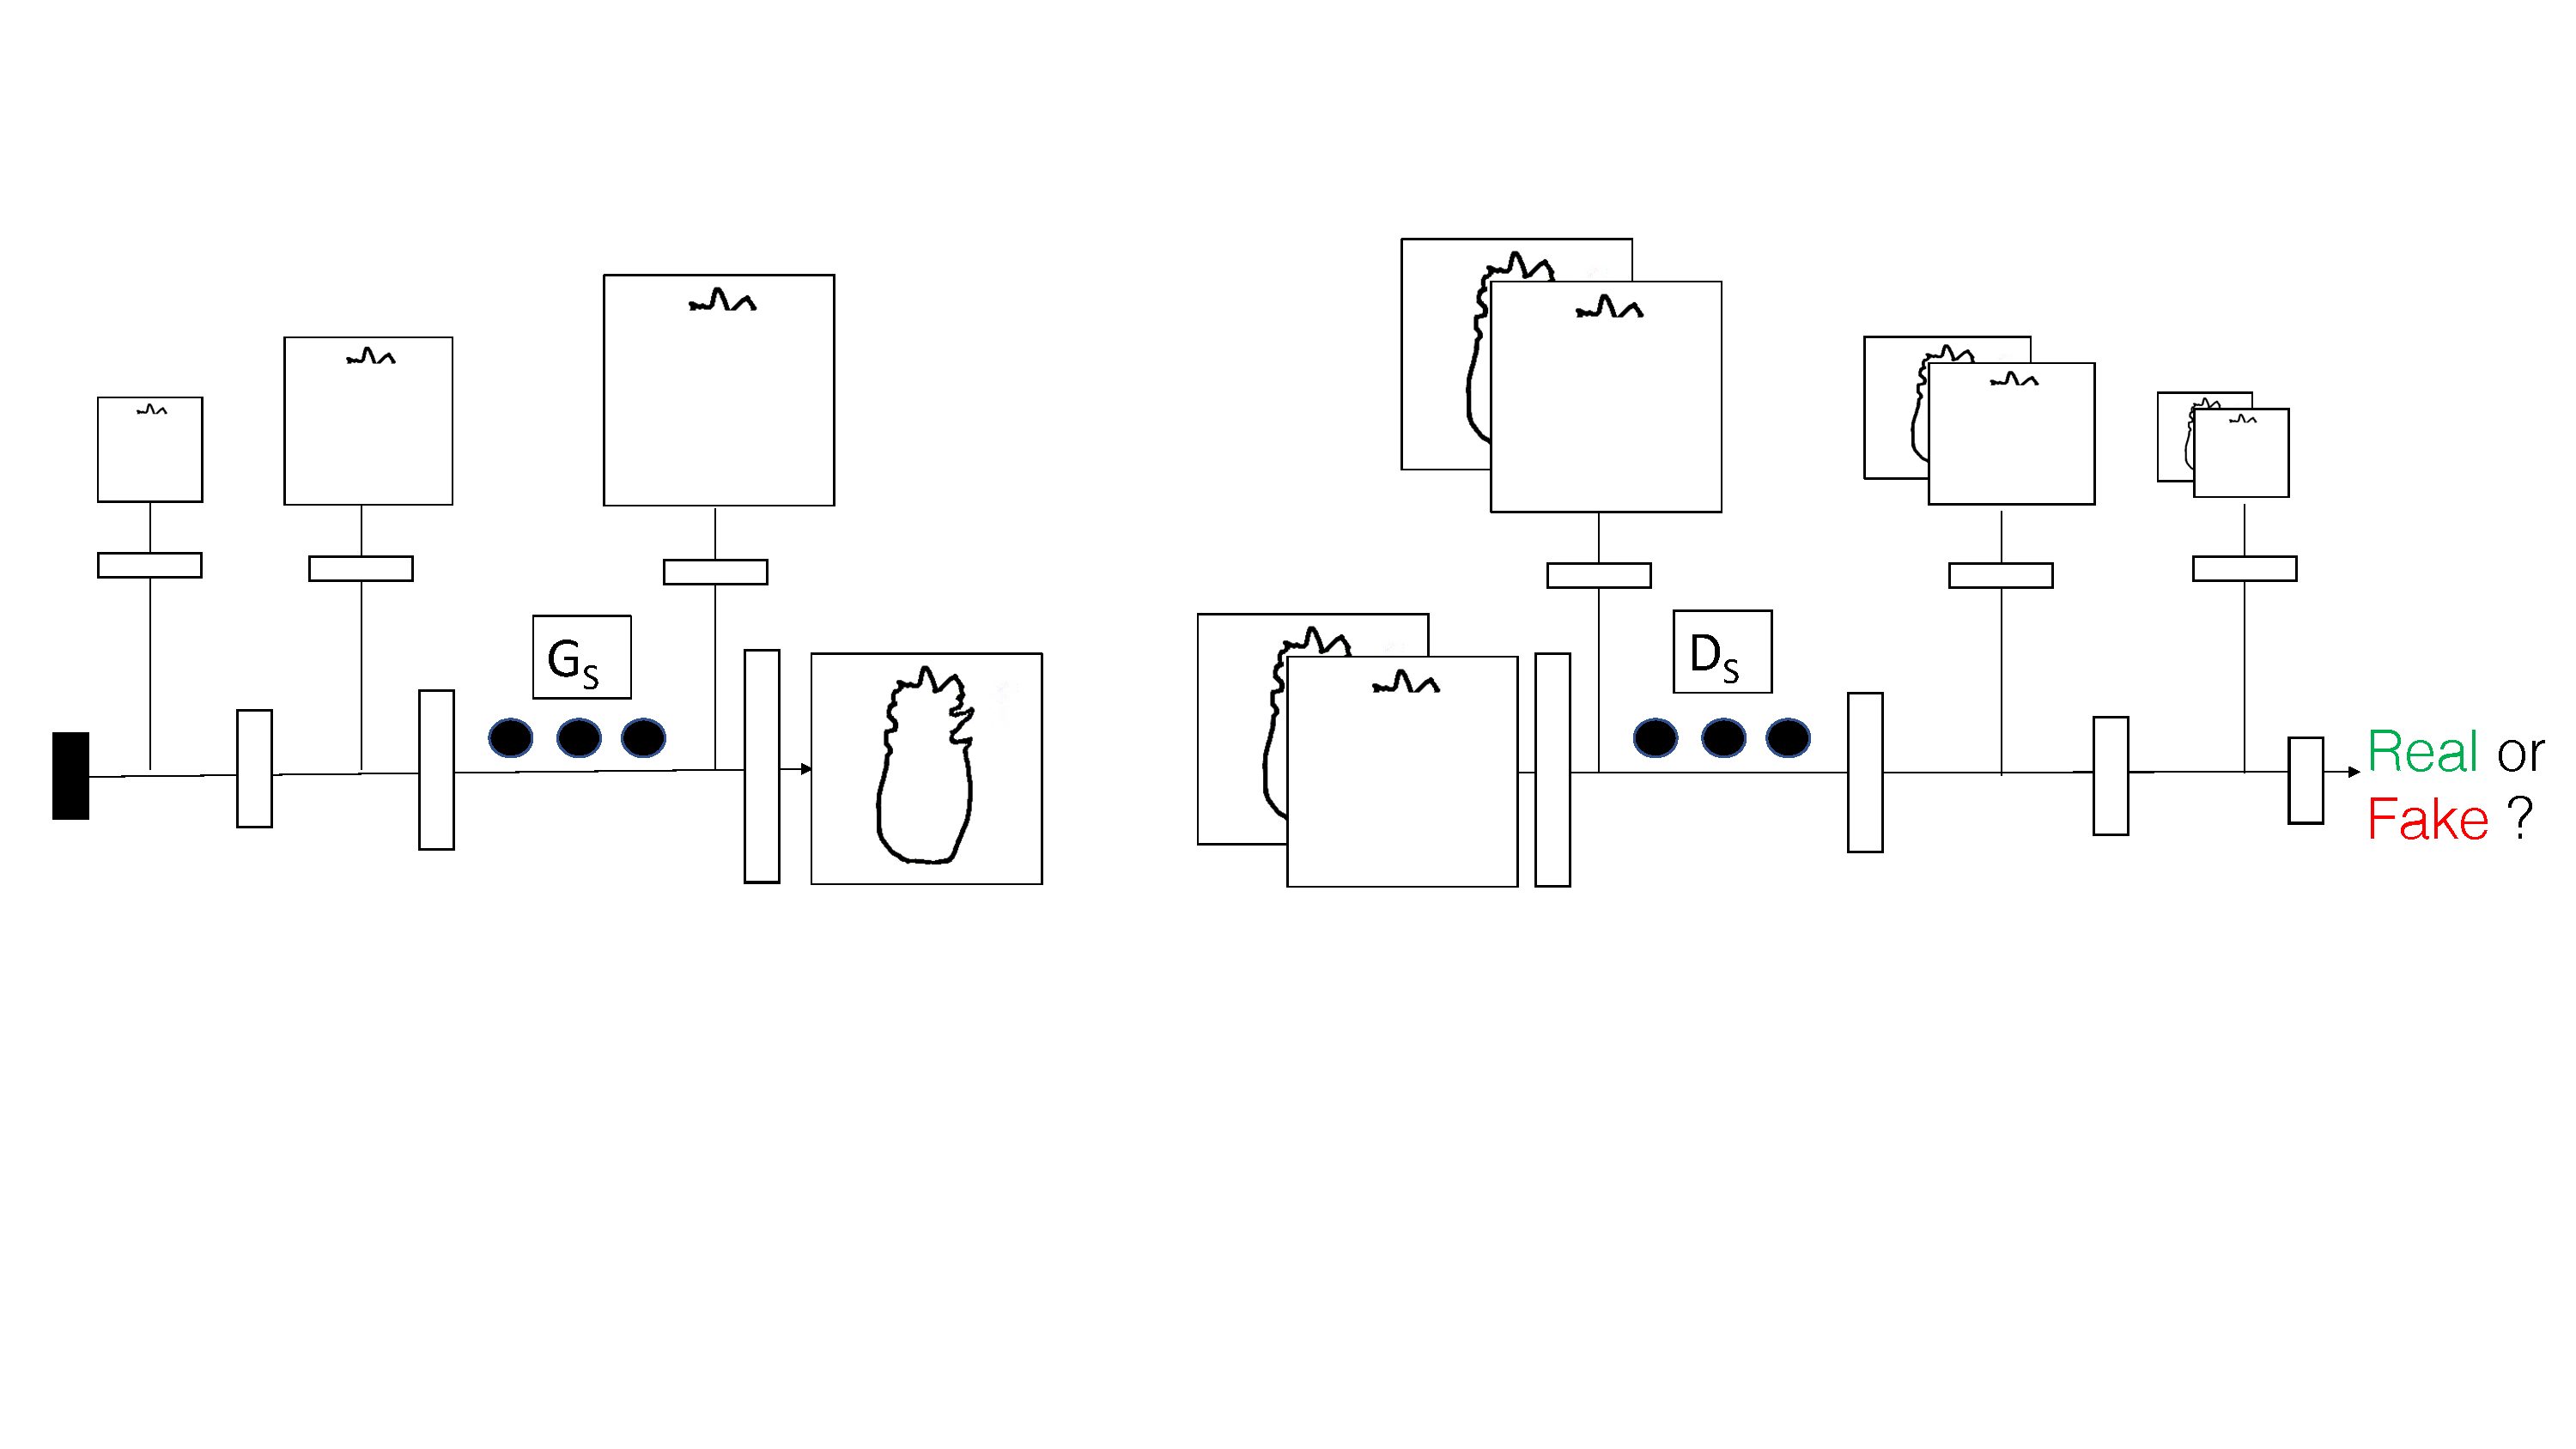
\includegraphics[width=\linewidth]{images/shape_completion/shape_completion.pdf}
    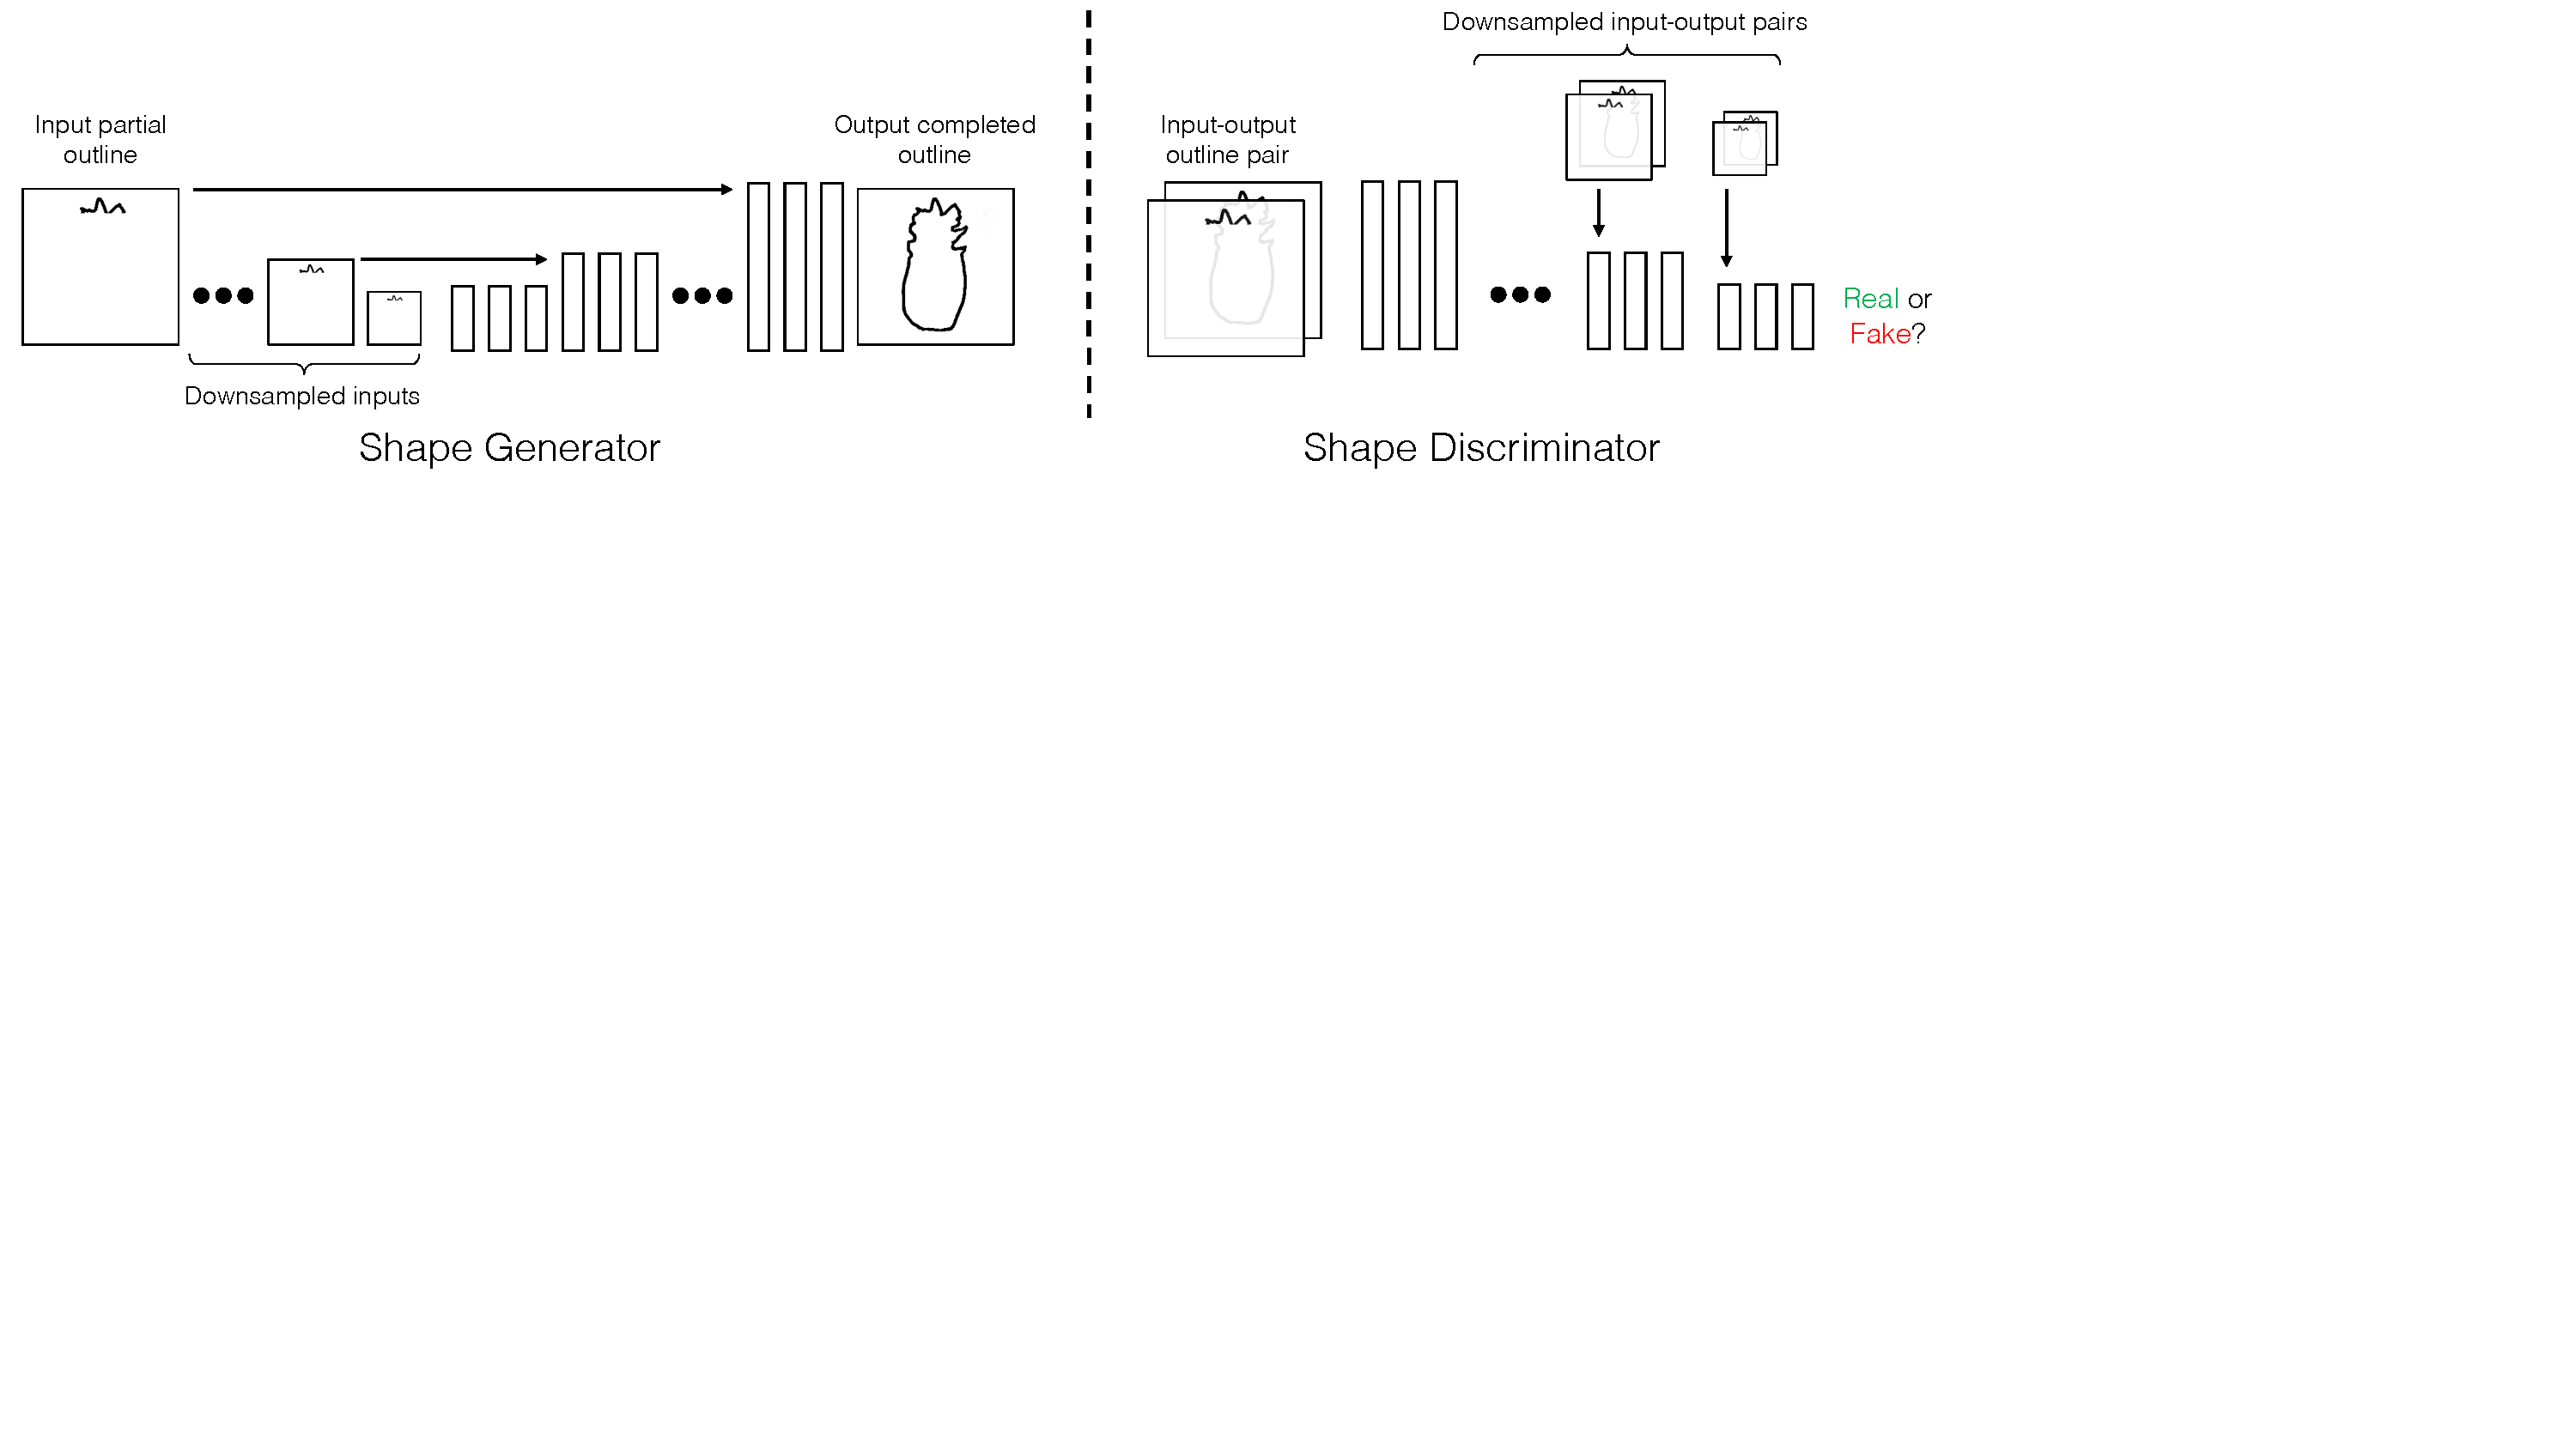
\includegraphics[width=\linewidth]{paper_images/arch_shape.pdf}
    \caption{\textbf{First stage: Shape Generator}: To achieve multi-modal completions $G_S$ design inspired from unconditional generator, with the conditioning provided at multiple scales to $G_S$ and $D_S$
    }\label{fig:SketchNet}
    %\vspace{-2mm}
\end{figure*}

\label{sec:methods}


% \section{Methodology (New)}
% First talk about the two inherent problems: partial (interactive) to full (task1), and outline to image (task2). mention that jointly training didn't work, analysis provided in the experiment section, so we go for two stage training. One potential reason for the joint training to fail would be that task1 requires understanding category-specific geometry and task2 requires filling the category-specific texture. Learning both jointly is difficult.

% \subsection{Interactive partial to full outline completion}
% \begin{itemize}
%     \item simple approach, data-driven, multiple partials to single full outline
%     \item used Bicycle GAN
%     \iten works surprisingly well
% \end{itemize}

% \subsection{Outline to real image synthesis}
% \begin{itemize}
%     \item Again, used GAN. objective is to train one GAN for multiple object categories
%     \item naive approach didn't work as conditioning seemed not that informative, mixed multiple categories together, bad results
%     \item used gating as it helps network to focus on the parts (or activations) of the network specific to  the features needed for a given category
%     \item just show the gating figure, explain what is means when it comes to modifying the architecure 
%     \item mention that there is information theoretic properties as well which you will discuss in the following subsection (refer)
% \end{itemize}

% \subsection{Insights on gatings}
% \begin{itemize}
%     \item put the mutual information based intuition (not sure)
%     \item mention that just to verify this, you trained infoGAN with gating on image to image and surprisingly it produced diverse generations which otherwise requires sophisticated and well thought models such as BicycleGAN, MAD-GAN etc
%     \item you can also talk about the 1D experiments here
% \end{itemize}

\section{Method}
We decouple the problem of interactive image generation into two stages: object shape completion from sparse user sketches, and appearance synthesis from the completed shape. More specifically as illustrated in \figref{fig:SketchFillNet} we use the Shape Generator $G_S$ for the automatic shape (outline/sparse sketch) generation and the Appearance Generator $G_A$ for generating the final image as well as the adversary discriminators $D_S$ and $D_A$. The method can be seen effective in the user interface in \figref{fig:gui}.
%To ensure that the generated shape completions and appearance completions are accurate for their respective domains we use the Shape Discriminator $D_S$ and the Appearance Discriminator $D_A$.
% \es{we need to refer to Fig.~\ref{fig:SketchFillNet} and use it's terminology $G_S$, $G_A$, ...}
%A naive method of bypassing this two step process and generating the final image from the partial strokes yielded sub-par results demonstrated in Section \ref{sec:experiments} hence necessitating the 2 step process. 
%A potential reason for the failure of the direct process is because it requires understanding category-specific geometry and the category-specific texture. Learning both jointly is difficult.

\subsection{Shape completion}
\label{sec:shape}
The shape completion network $G_S$ should provide the user with a visualization of its  completed shape, based on user input, and should keep on updating the suggested shape interactively. 
%For an interactive user interface to be effective, the network has to generate an estimated full image shape as the user adds sparse input. 
We take a data-driven approach for this whereby, to train the network, we simulate partial strokes by removing random square patches from the full outline/ full sparse sketch image. 
The patches are of three sizes (64$\times$64, 128$\times$128, 192$\times$192) and are placed at a random location in the image (of size 256$\times$256). An illustration can be seen in \figref{fig:autocomplete_data_generation}.
% \es{probably need more details here - size of squares, how many per image, total training data size etc.}
We automatically generate data in this manner creating a dataset where 75 different partial outlines/sketches are created from a single outline/sketch image.
%We found that the BicycleGAN model~\cite{zhu2017toward} performed well on the shape completion task, and we train it, unmodified, on pairs of partial-full outline images. %(Fig.~\ref{fig:infogan_gate}, top left).
The model used to generate multimodal completions of the input sketch is depicted in \figref{fig:SketchNet} based on the architecture used for non-image conditional generations in \cite{mescheder2018training}. We modify the architecture such that the conditioning input scribble is provided to the generator and discriminator at multiple scales. 



\begin{figure}[t]
\centering
\begin{tabular}{*{4}{c@{\hspace{3px}}}}
    \frame{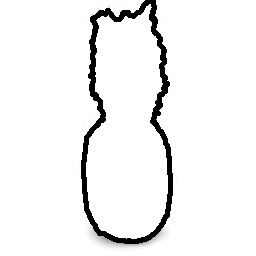
\includegraphics[width=.22\linewidth]{images/autocomplete_data_generation/original.png}} &
    \frame{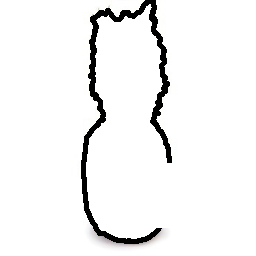
\includegraphics[width=.22\linewidth]{images/autocomplete_data_generation/64.png}} &
    \frame{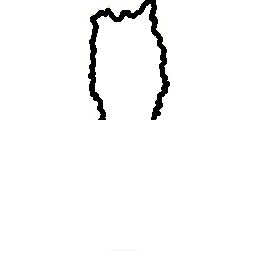
\includegraphics[width=.22\linewidth]{images/autocomplete_data_generation/128.png}} &
    \frame{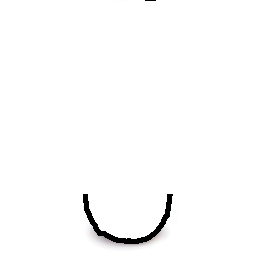
\includegraphics[width=.22\linewidth]{images/autocomplete_data_generation/192.png}}\\
    Outline &
    64$\times$64&
    128$\times$128 &
    192$\times$192\\
\end{tabular} \\
    \caption{\textbf{Autocomplete Simulated Inputs:} 3 sizes (64$\times$64,128$\times$128,192$\times$192) of white colored occluders were used for simulating partial edges.}
    \label{fig:autocomplete_data_generation}
\end{figure}

\begin{figure*}[t]
    \centering
    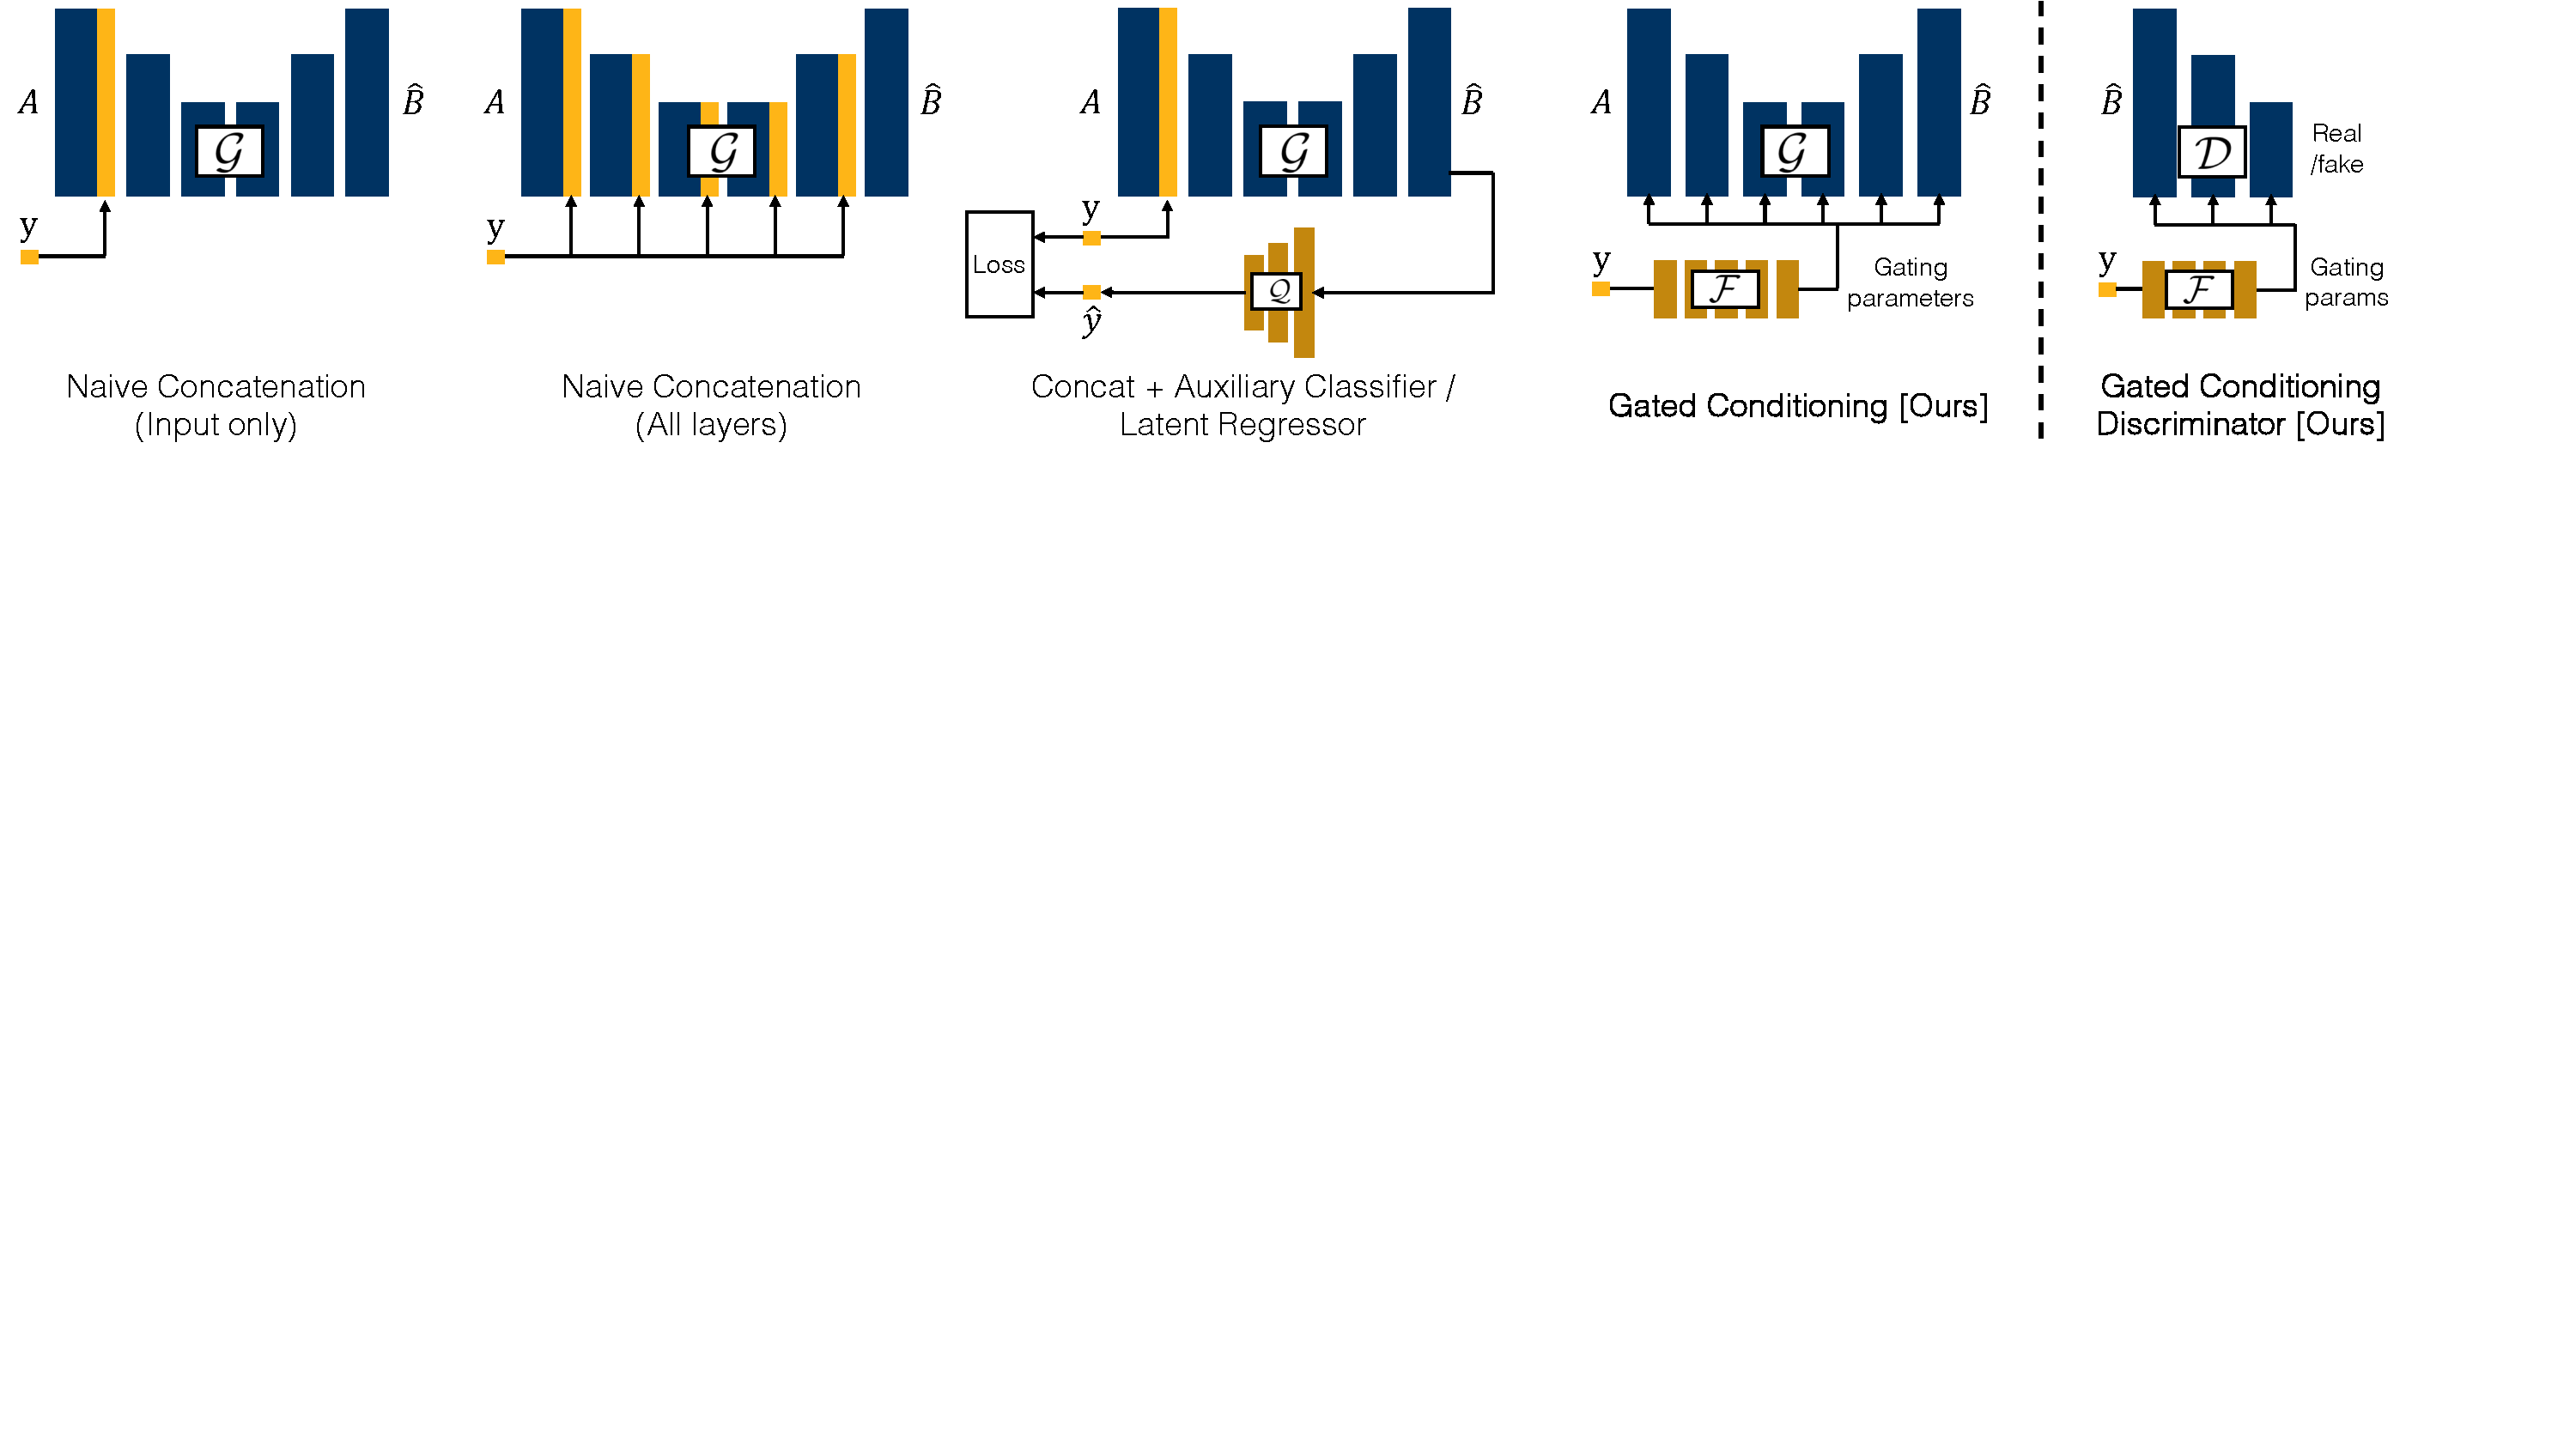
\includegraphics[width=1.\linewidth]{paper_images/arch_inject2.pdf}
    \caption{
    \vspace{-2mm}
    {\bf Conditioning variants for the Appearance Generator} \label{fig:arch-gate}
    \vspace{-2mm}
    }
\end{figure*}

\begin{figure*}[t]
    \centering
    % 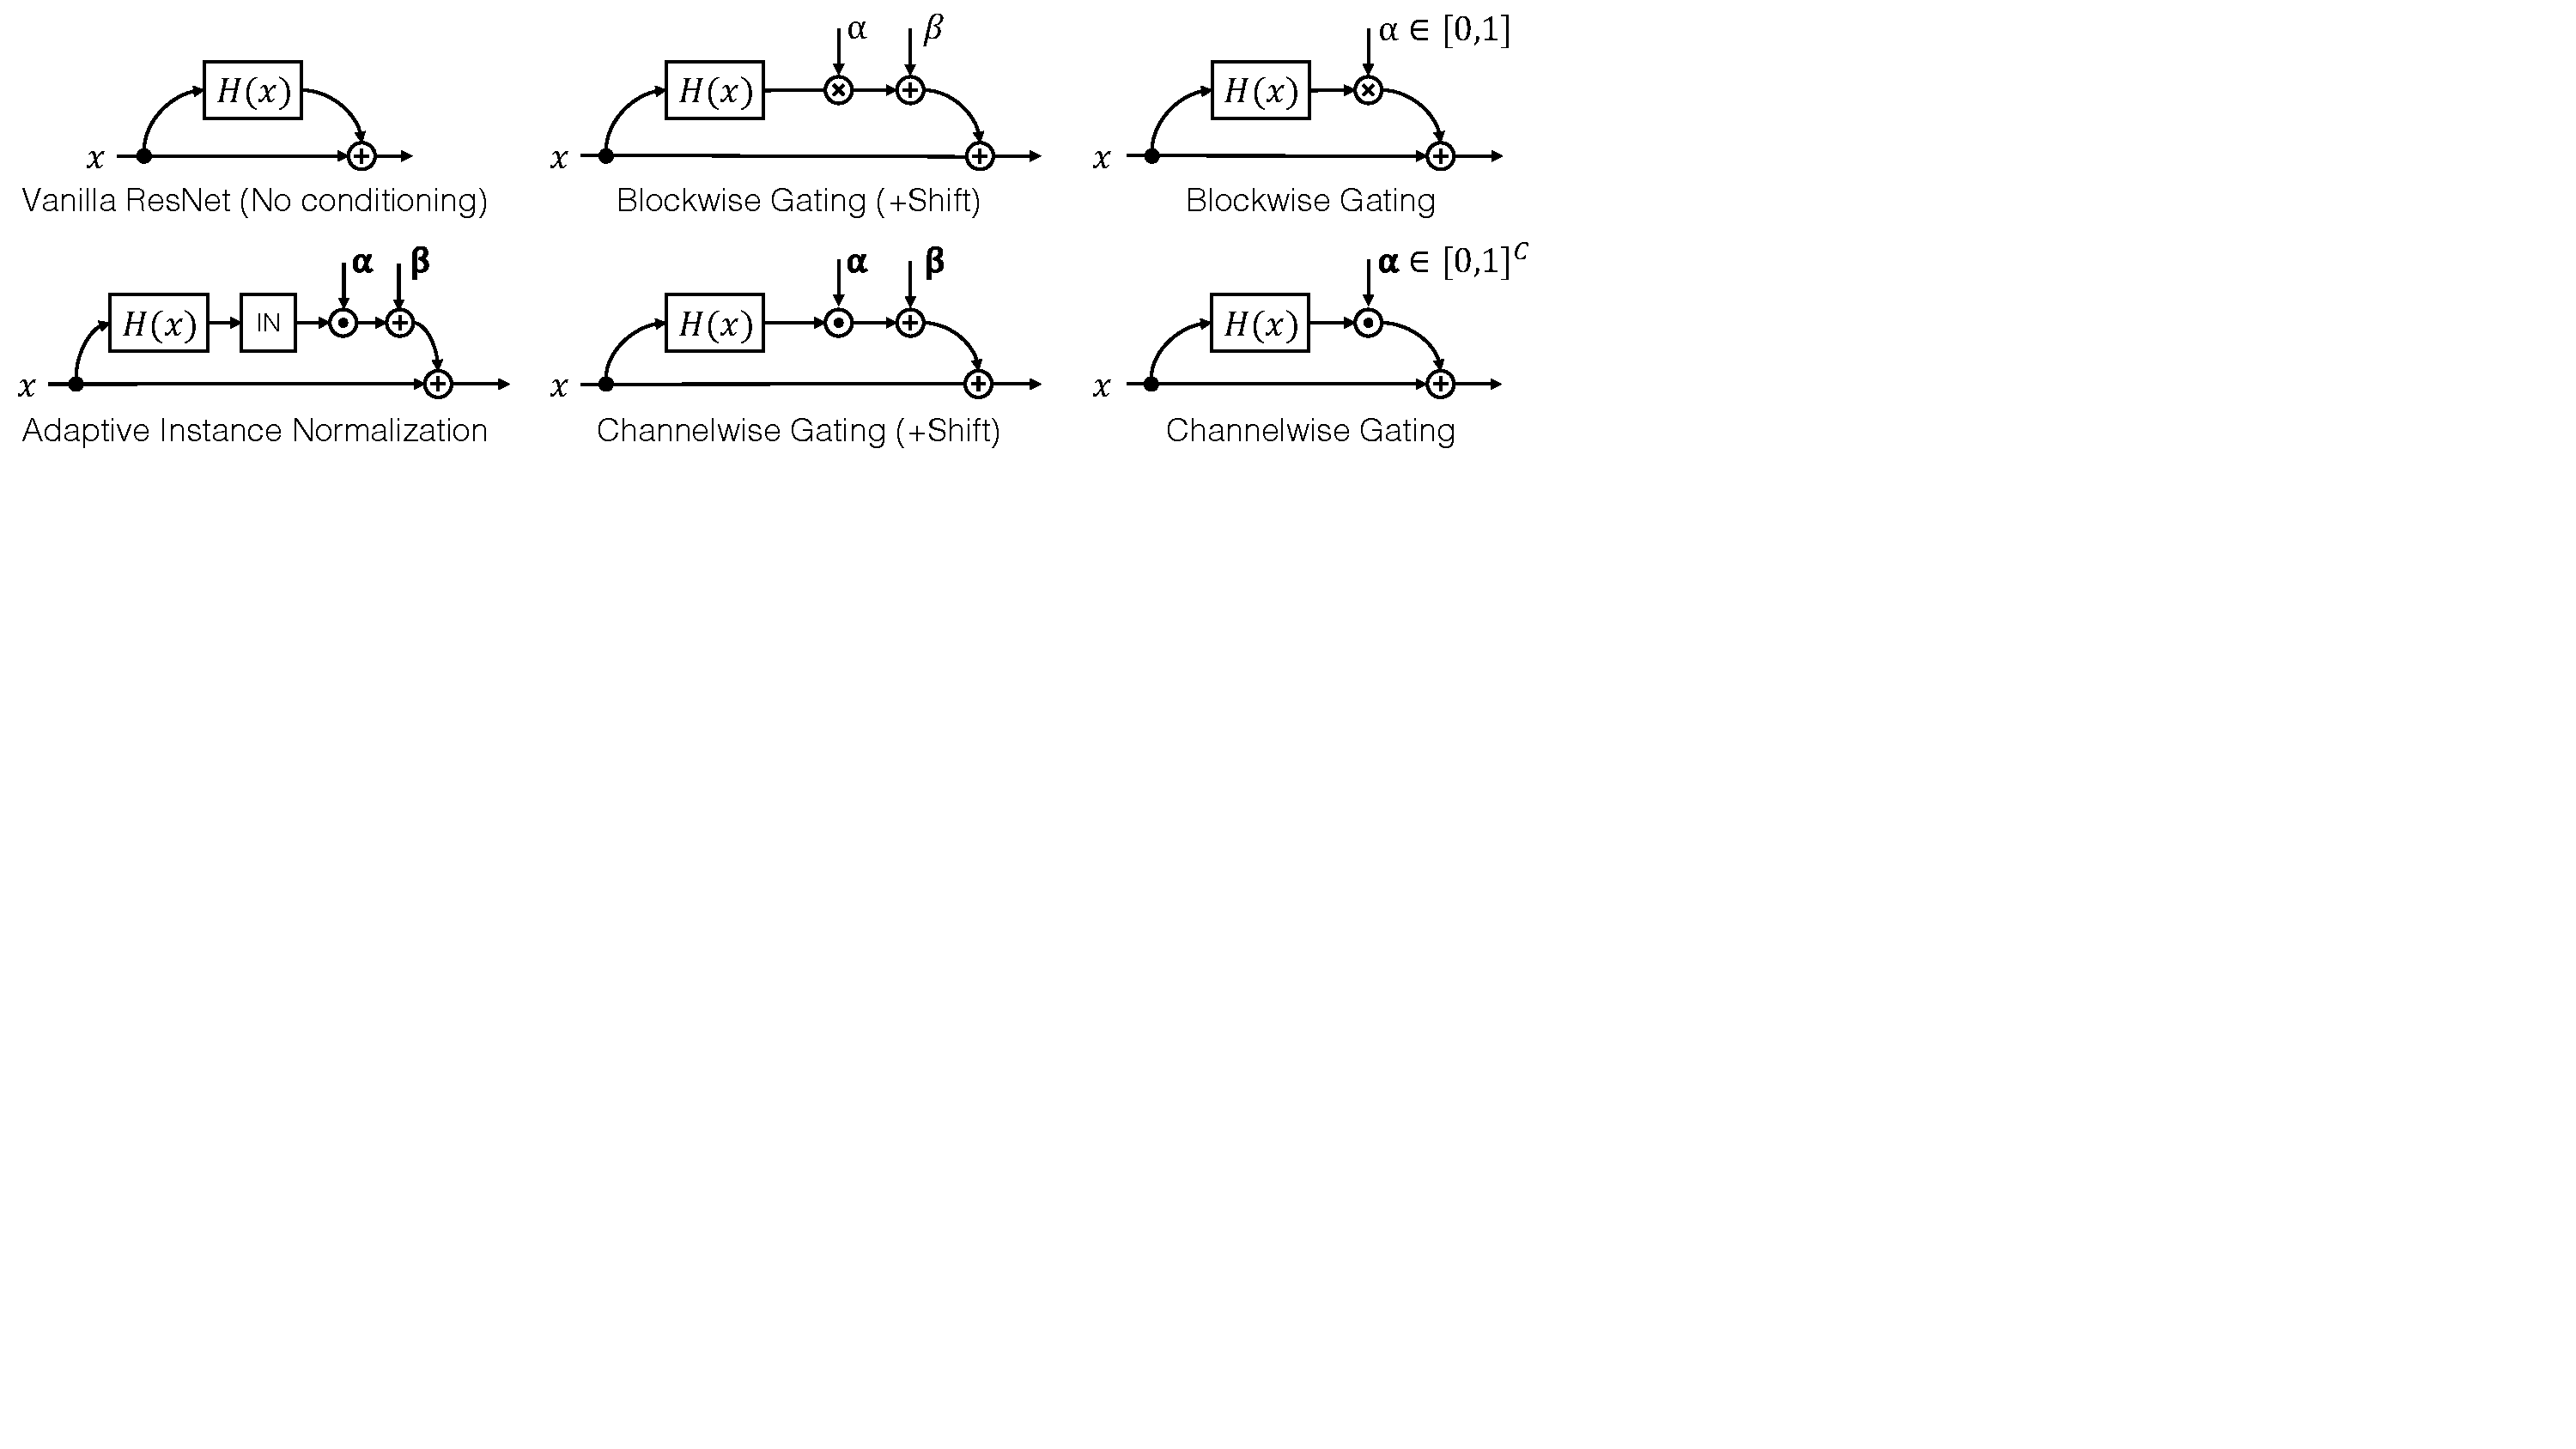
\includegraphics[width=\linewidth]{paper_images/arch_gate.pdf}
    % 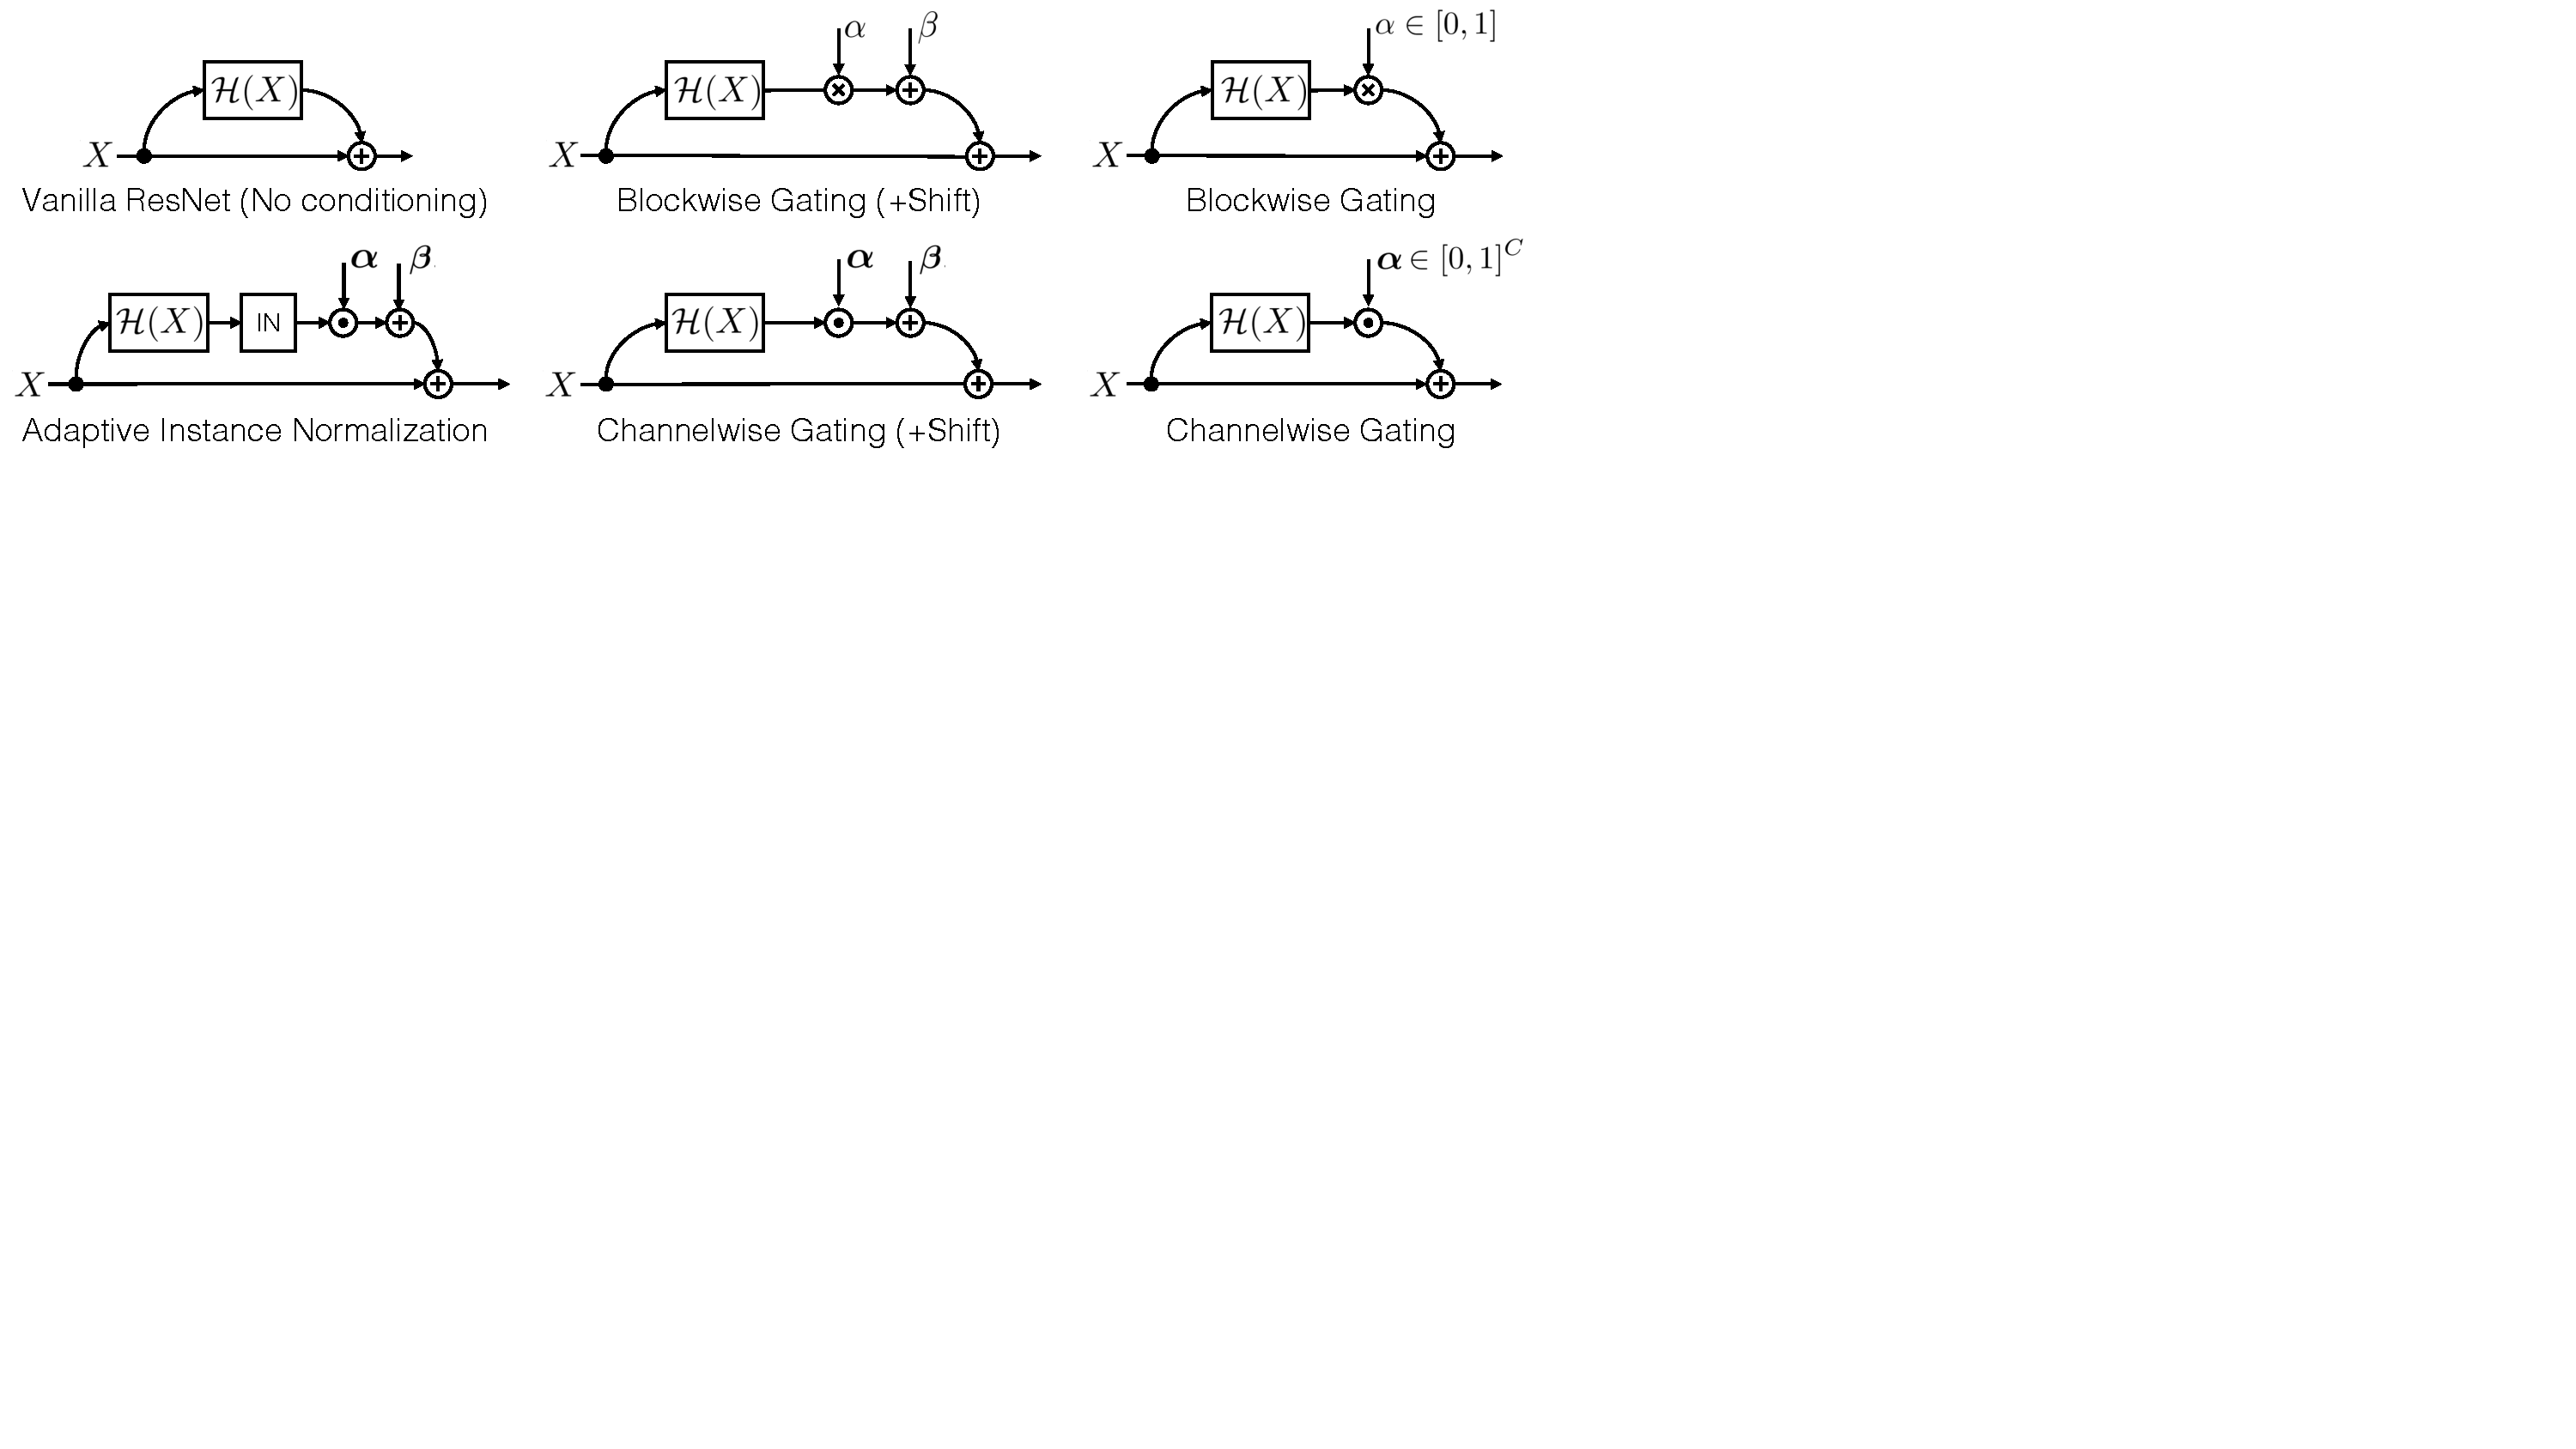
\includegraphics[width=.9\linewidth]{paper_images/arch_gate2.pdf}
    % \caption{
    % % {\bf Incorporating soft-gating into residual blocks.} \rz{Order got changed, may or may not need to add key for hadamard product}
    % {\bf (Top-left)} A ``vanilla" residual block without conditioning modifies input tensor $X$ into $X+\mathcal{H}(X)$. Conditioning with concatenation uses this setup. {\bf (Top-mid)} The $\mathcal{H}(X)$ block is softly-gated by scalar parameter $\alpha$ and shift $\beta$. {\bf (Top-right)} Only the gating is used, without bias. {\bf (Bot-left)} Adaptive Instance Normalization~\cite{huang2017arbitrary} applies a channel-wise scaling and shifting after an instance normalization layer. {\bf (Bot-mid)} Channel-wise gating adds restrictions to the range of $\mbox{\boldmath $\alpha$}$. {\bf (Bot-right)} We find empirically, that channel-wise gating (without added bias) produced the best results.\label{fig:arch-gate}
    % \vspace{-2mm}
    % }
    % \vspace{-4mm}
    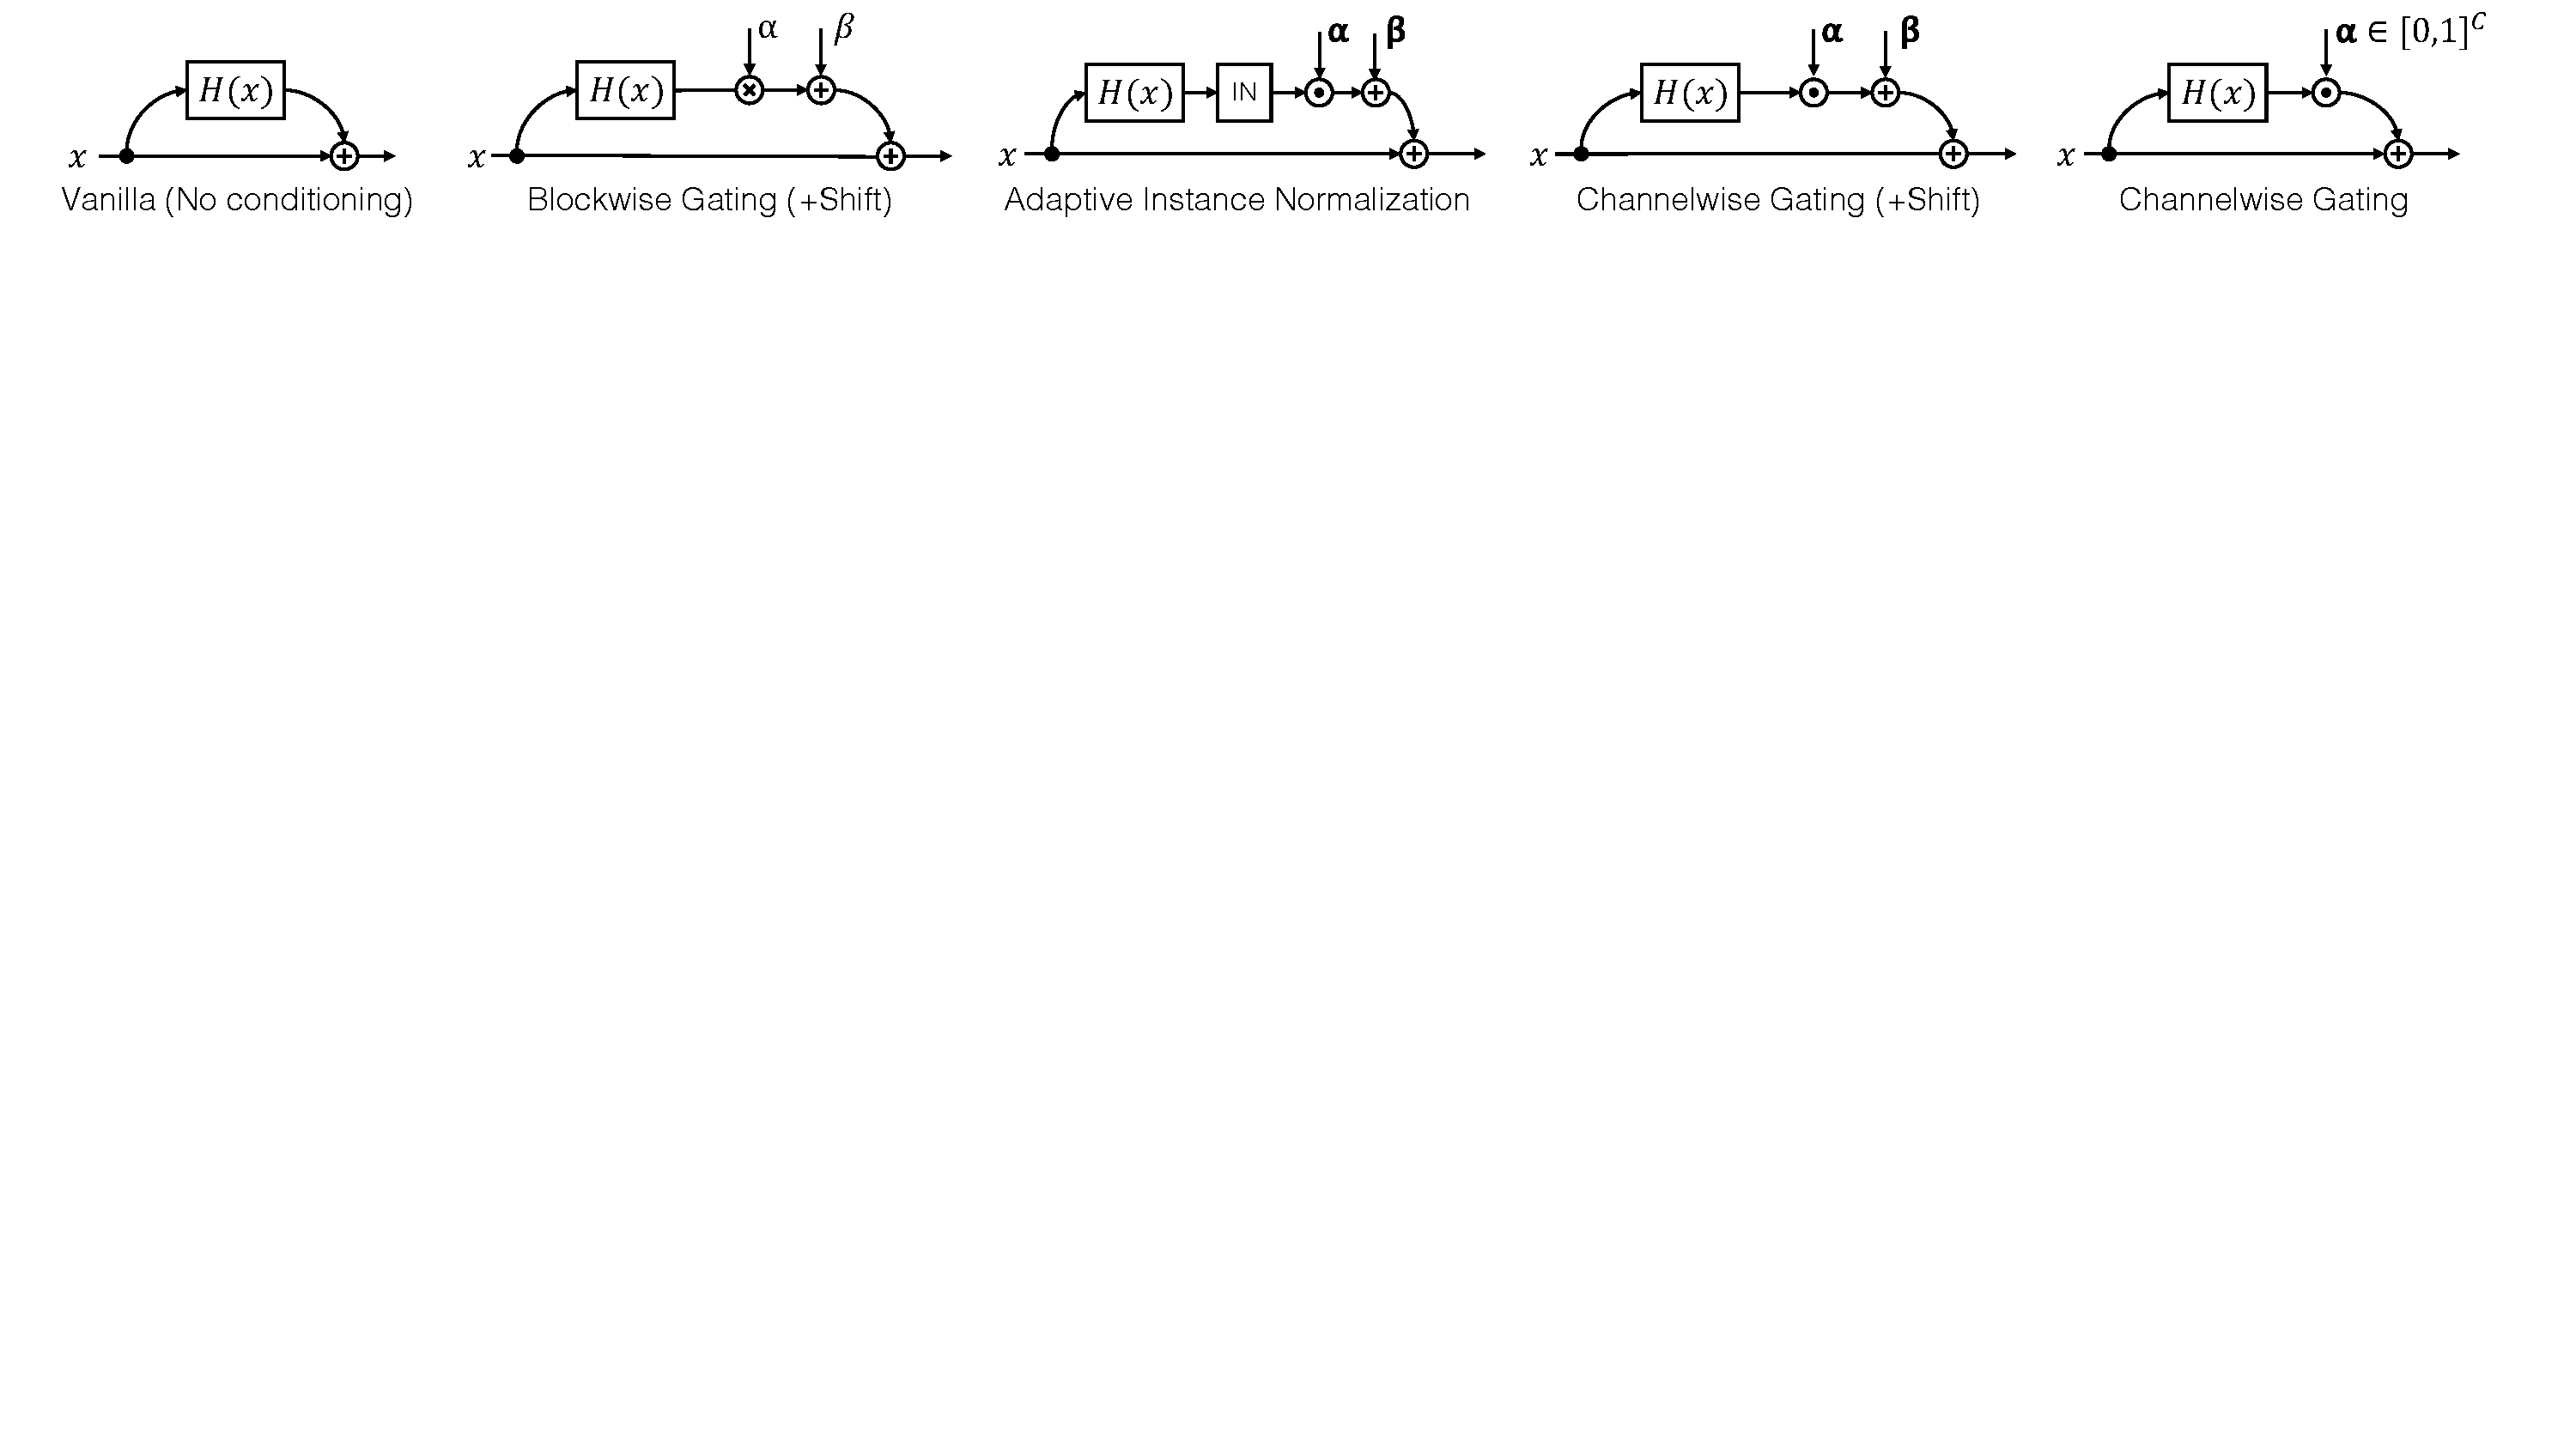
\includegraphics[width=1.\linewidth]{paper_images/arch_gate3.pdf}
    \caption{
    % {\bf Incorporating soft-gating into residual blocks.} \rz{Order got changed, may or may not need to add key for hadamard product}
    {\bf Injecting conditioning with modified residual layers} {\bf (Left)} A ``vanilla" residual block without conditioning applies a residual modification to the input tensor. {\bf (Mid-left)} The $\mathcal{H}(X)$ block is softly-gated by scalar parameter $\alpha$ and shift $\beta$. {\bf (Mid)} Adaptive Instance Normalization~\cite{huang2017arbitrary} applies a channel-wise scaling and shifting after an instance normalization layer. {\bf (Mid-right)} Channel-wise gating adds restrictions to the range of $\mbox{\boldmath $\alpha$}$. {\bf (Right)} We find empirically, that channel-wise gating (without added bias) produced the best results.\label{fig:arch-gate}
    \vspace{-2mm}
    }
\end{figure*}


\begin{figure*}[t]
    \centering
    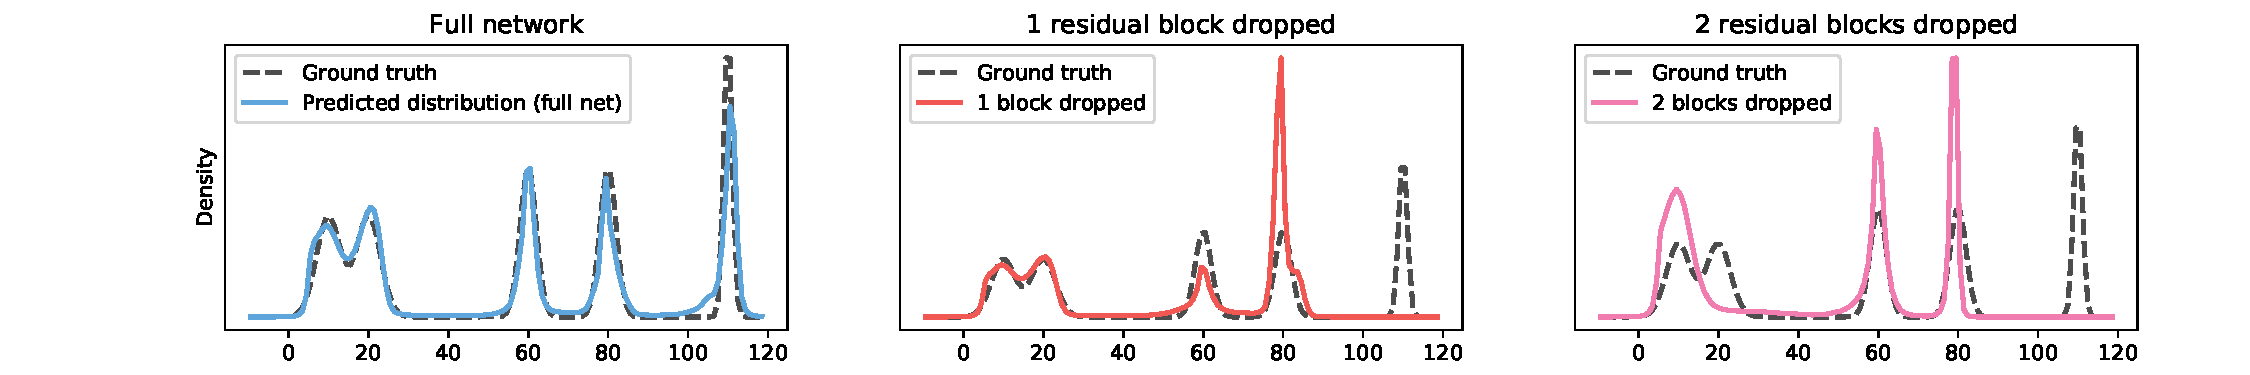
\includegraphics[width=\linewidth,trim={2.6cm 0 1.8cm 0},clip]{paper_images/mog.pdf}
    % 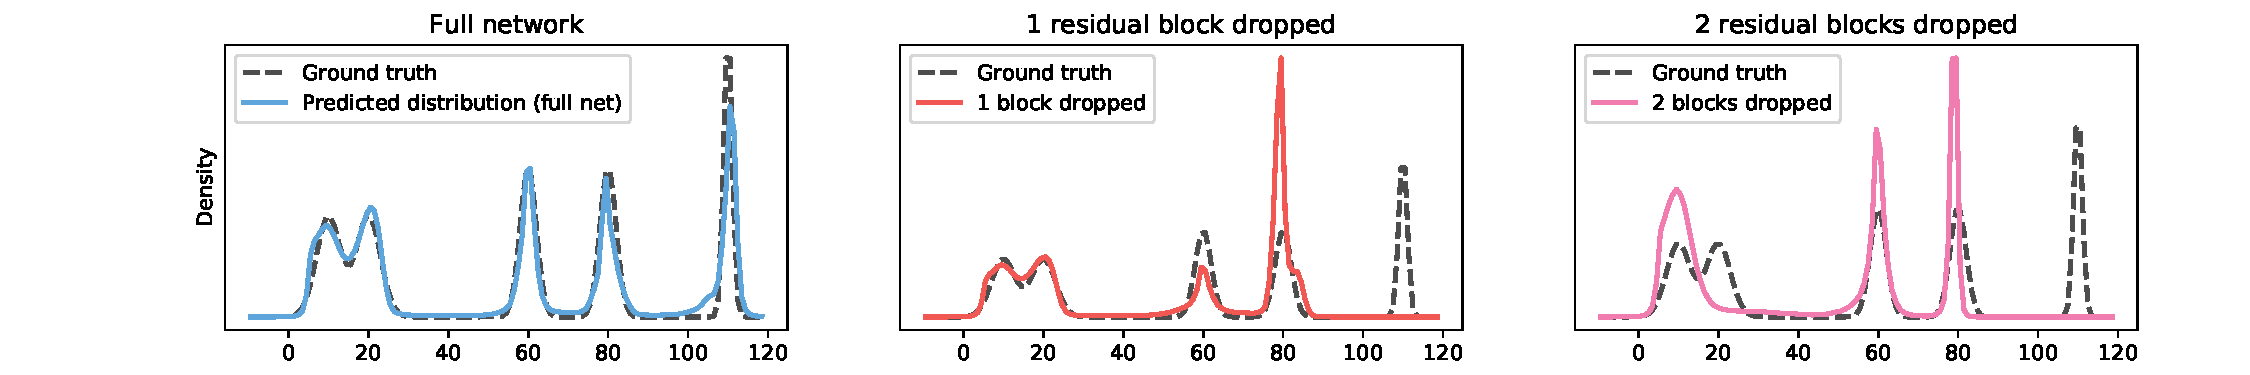
\includegraphics[width=\linewidth]{paper_images/mog.pdf}
    \caption{{\bf 1D Mixture of Gaussians.} {\bf (Left)} Samples from a residual network (blue-dotted) closely approximate the training distribution (black). {\bf (Mid)} Removing one residual block removes one mode of the predicted distribution. {\bf (Right)} Removing two blocks drops two modes. Note that samples stay mostly ``on-manifold" of the ground truth distribution.
    %\vspace{-2mm}
    }\label{fig:onedexperiment}
    %\vspace{-3mm}
\end{figure*}

\subsection{Appearance synthesis}
\label{sec:appearance}
%We use a conditional GAN formulation for generating images from outlines as shown by the efficacy in \cite{isola2016image2image,zhu2017toward}. 
An ideal interactive sketch-to-image system  should be able to generate multiple different image classes with a single generator. 
Beside memory and time considerations (avoiding loading/using a separate model per class, reducing overall memory), a single network can share features related to outline recognition and texture generation that are common across classes, which helps training with limited examples per class. %\es{Didn't we already said that in the intro? If yes we should remove/significantly shorten}

As we later show, existing class conditioning-by-concatenation techniques fail to properly condition the network about the class information in current image translation networks~\cite{isola2016image2image,zhu2017toward}.
%
To address this, we propose an effective soft gating mechanism, shown in Figure~\ref{fig:arch-gate}.
Conceptually, our network consists of a small external gating network that is conditioned on the object class (encoded as a 1-hot vector).
The gating network outputs parameters that are used to modify the features of the main generator network.
We now describe this architecture in detail.
%condition the main generator 
%control the bias and/or amount of activation of different layers/channels in a fully ResNet generation network~\cite{he2016deep} with added ResNet-like upsampling and downsampling layers. 
% Similar to \cite{karras2018style} we used a soft gating mechanism to properly condition the generator about the class condition using a gating hypernetwork which generated a map of how to use the various residual blocks based on the class conditioning. As shown in \figref{fig:arch-inj} we have all the layers implemented as resnet blocks and the gating hypernetwork decides how much ($\alpha$) of each block $f(x)$ to use via a simple gate $\alpha$ for a block i.e. the output of each block is now $x + \alpha f(x)$  where $\alpha \in [0,1]$. We explored certain variations of the above technique by introducing gating in the discriminator as well as generalizing from block-wise gating to channel-wise gating. For a complete analysis of the various forms of gating please refer to the supplementary material.
%
%The methods above do not fundamentally modify the structure of the network. 
In ResNets~\cite{he2016deep}, an input feature tensor $X_l$ is modified by function
\begin{equation}
X_{l+1} = X_l+\mathcal{H}_l(X_l).
\end{equation}
Changes in resolution are obtained by upsampling before or downsampling after the residual block.
%We investigate multiple variants of the \textit{learned} gating network.
% , as illustrated in Fig.~\ref{fig:arch-gate}.
% For visual clarity, we omit the layer subscript $l$ in feature tensor $X_l$, residual subnetwork $\mathcal{H}_l$, and the gating parameters $\alpha_l, \beta_l$.
Note that we're omitting "l" subscript for clarity.
Our gating network augments this with a predicted scalar $\alpha$ for each layer of the network using a learned network $\mathcal{F}({\bf y})$, where  ${\bf y}$ is the conditioning vector:
\begin{equation}
X + \alpha \; \mathcal{H}(X), \text{where } \alpha \in [0,1]
\end{equation}

If the conditioning vector ${\bf y}$ has no use for a particular block, it can predict $\alpha$ close to zero and effectively switch off the layer.
% , and use that layer instead for other classes.
During training, blocks within the main network can transform the image in various ways, and $\mathcal{F}$ can modulate such that the most useful blocks are selected. 
Unlike previous feature map conditioning methods such as AdaIn~\cite{ulyanovinstance}, we apply gating to \emph{both} the generator and discriminator. 
This enables the discriminator to select blocks which effectively judge whether generations are real or fake, conditioned on the class input.
% Via accurate gradients backpropagated to the generator it also enables the generator to generate class conditioned high resolution image samples.
Some blocks can be shared across regions in the conditioning vector, whereas other blocks can specialize for a given class.

A more powerful method is to apply this weighting channel-wise using a vector {\boldmath$\alpha$}: % This is denoted as follows:
\begin{align}
X + \mbox{\boldmath $\alpha$} \odot \mathcal{H}(X), \text{where } \mbox{\boldmath $\alpha$} \in [0,1]^c 
\end{align}
Where $\odot$ represents channel-wise multiplication. This allows specific channels to be switched ``on" or ``off", providing additional degrees of freedom.
%We make the corresponding changes in the discriminator as well. 
%Soft-gating has been explored by Veit et al.~\cite{veit2018adaptive} in a classification setting. 
We found that this channelwise approach for gating provides the strongest results. 

We additionally explored incorporating a bias term after the soft-gating, either block-wise using a scalar $\beta \in [-1,1]$ per layer, or channel-wise using a vector $\mbox{\boldmath $\beta$} \in [-1, 1]^c$ per layer but we found that they did not help much, and so we leave them out of our final model.
% \ow{but found that they did not help much, and so we leave them out of our final model?}




Finally, we describe our network architecture. 
We base our architecture on the proposed residual \textbf{Encoder-Decoder} model from MUNIT~\cite{huang2018multimodal}.
This architecture is comprised of 3 \texttt{conv} layers, 8 residual blocks, and 3 \texttt{up-conv} layers. The residual blocks have 256 channels. 
First, we deepen the network, based on the principle that deeper networks have more valid disjoint, partially shared paths~\cite{veit2016residual}, and add 24 residual blocks. 
To enable the larger number of residual blocks, we drastically reduce the width to 32 channels for every layer. 
We refer to this network as \textbf{SkinnyResNet}. 
Additionally, we found that modifying the downsampling and upsampling blocks to be residual connections as well improved results, and also enables us to apply gating to {\em all} blocks. 
When gating is used, the gate prediction network, $\mathcal{F} ({\bf y})$,  
%Fig.~\ref{fig:arch-inj} (mid-right, right) 
is also designed using residual blocks. Additional architecture details are in the supplementary material. 

\begin{figure}[t]%[ht!]
\centering
\resizebox{1.0\linewidth}{!}{
\begin{tabular}{*{5}{c@{\hspace{3px}}}}
    \frame{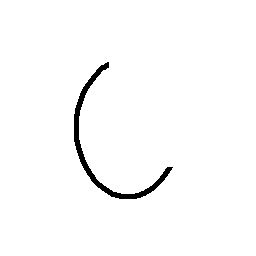
\includegraphics[width=.2\linewidth]{images/autocomplete_generate/scribble/basketball.png}} &
    %\frame{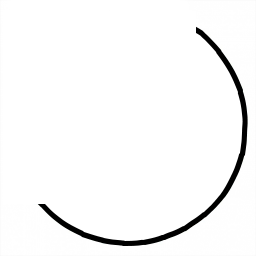
\includegraphics[width=.10\linewidth]{images/autocomplete_generate/scribble/soccer.png}} &
    \frame{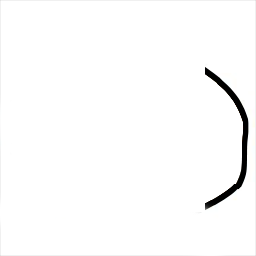
\includegraphics[width=.2\linewidth]{images/autocomplete_generate/scribble/watermelon.png}} & 
    \frame{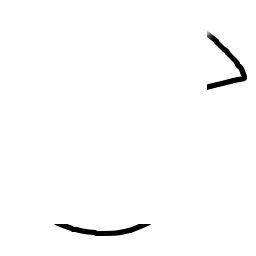
\includegraphics[width=.2\linewidth]{images/autocomplete_generate/scribble/orange.png}}&
    \frame{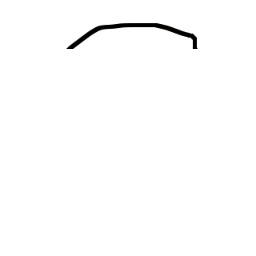
\includegraphics[width=.2\linewidth]{images/autocomplete_generate/scribble/cookie.png}} &
    %\frame{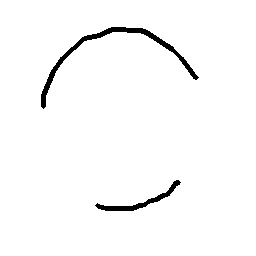
\includegraphics[width=.10\linewidth]{images/autocomplete_generate/scribble/moon.png}} &
    %\frame{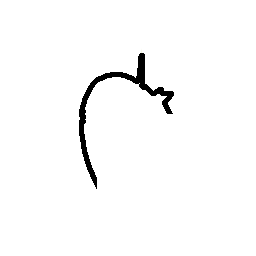
\includegraphics[width=.10\linewidth]{images/autocomplete_generate/scribble/strawberry.png}} &
    \frame{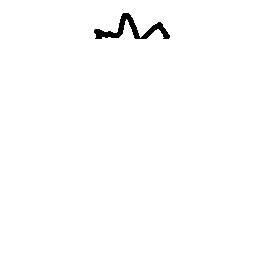
\includegraphics[width=.2\linewidth]{images/autocomplete_generate/scribble/pineapple.png}}
    %\frame{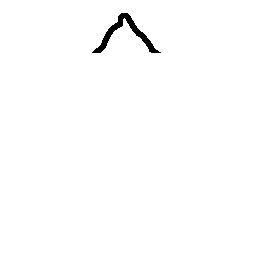
\includegraphics[width=.10\linewidth]{images/autocomplete_generate/scribble/cupcake.png}} &
    %\frame{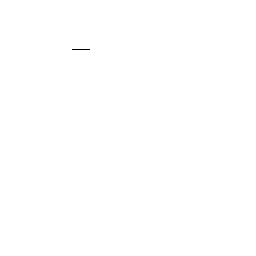
\includegraphics[width=.10\linewidth]{images/autocomplete_generate/scribble/chicken.png}}
    \\
    
    \frame{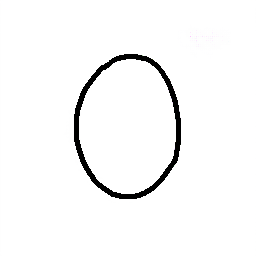
\includegraphics[width=.2\linewidth]{images/autocomplete_generate/autocomplete/basketball.png}} &
    %\frame{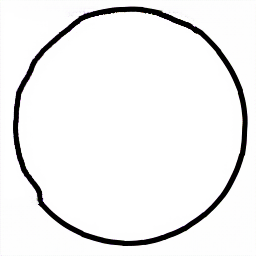
\includegraphics[width=.10\linewidth]{images/autocomplete_generate/autocomplete/soccer.png}} &
    \frame{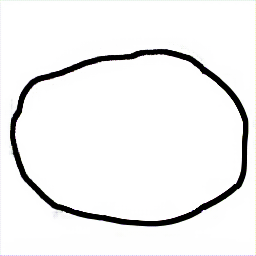
\includegraphics[width=.2\linewidth]{images/autocomplete_generate/autocomplete/watermelon.png}} & 
    \frame{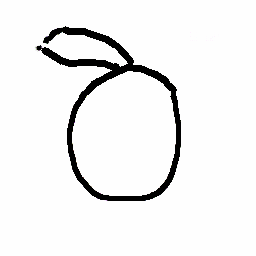
\includegraphics[width=.2\linewidth]{images/autocomplete_generate/autocomplete/orange.png}}&
    \frame{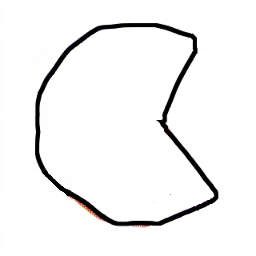
\includegraphics[width=.2\linewidth]{images/autocomplete_generate/autocomplete/cookie.png}} &
    %\frame{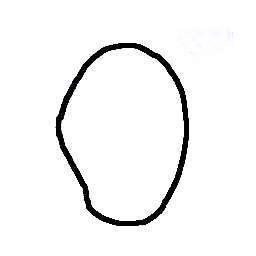
\includegraphics[width=.10\linewidth]{images/autocomplete_generate/autocomplete/moon.png}} &
    %\frame{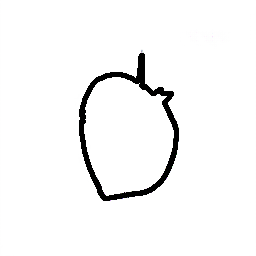
\includegraphics[width=.10\linewidth]{images/autocomplete_generate/autocomplete/strawberry.png}} &
    \frame{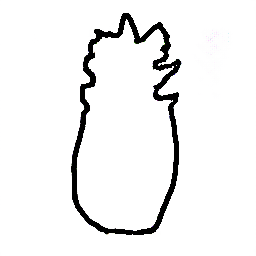
\includegraphics[width=.2\linewidth]{images/autocomplete_generate/autocomplete/pineapple.png}}
    %\frame{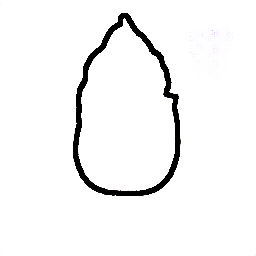
\includegraphics[width=.10\linewidth]{images/autocomplete_generate/autocomplete/cupcake.png}} &
    %\frame{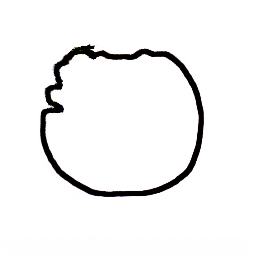
\includegraphics[width=.10\linewidth]{images/autocomplete_generate/autocomplete/chicken.png}}
    \\
    
    
    \frame{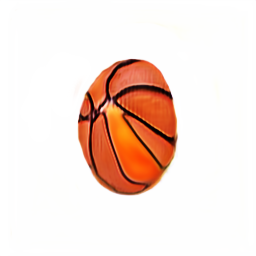
\includegraphics[width=.2\linewidth]{images/autocomplete_generate/image/basketball.png}} &
    %\frame{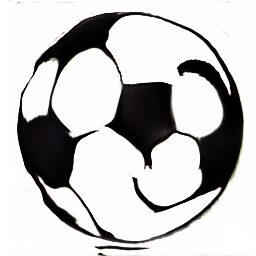
\includegraphics[width=.10\linewidth]{images/autocomplete_generate/image/soccer.png}} &
    \frame{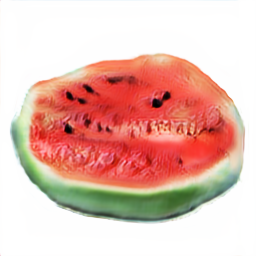
\includegraphics[width=.2\linewidth]{images/autocomplete_generate/image/watermelon.png}} & 
    \frame{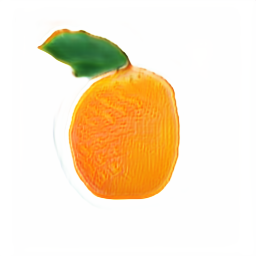
\includegraphics[width=.2\linewidth]{images/autocomplete_generate/image/orange.png}}&
    \frame{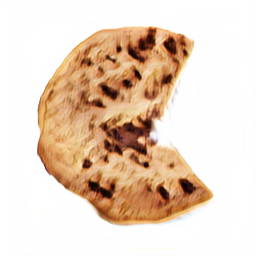
\includegraphics[width=.2\linewidth]{images/autocomplete_generate/image/cookie.png}} &
    %\frame{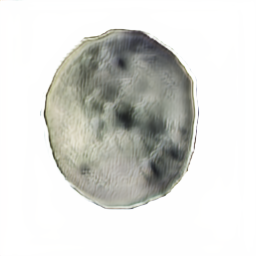
\includegraphics[width=.10\linewidth]{images/autocomplete_generate/image/moon.png}} &
    %\frame{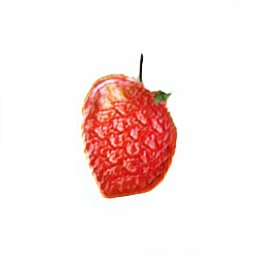
\includegraphics[width=.10\linewidth]{images/autocomplete_generate/image/strawberry.png}} &
    \frame{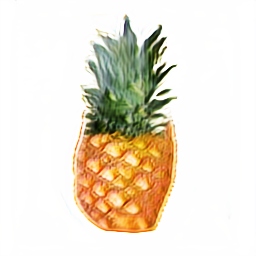
\includegraphics[width=.2\linewidth]{images/autocomplete_generate/image/pineapple.png}}
    %\frame{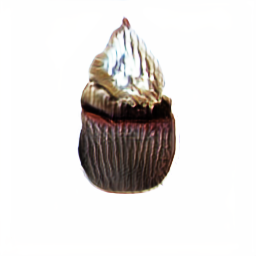
\includegraphics[width=.10\linewidth]{images/autocomplete_generate/image/cupcake.png}} &
    %\frame{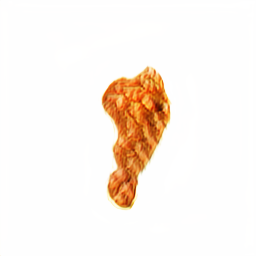
\includegraphics[width=.10\linewidth]{images/autocomplete_generate/image/chicken.png}}
    \\
    % \begin{subfigure}[t]{.15\linewidth}\caption{}\label{fig:basketball_partial}\end{subfigure} &
    % \begin{subfigure}[t]{.15\linewidth}\caption{}\label{fig:basketball_full}\end{subfigure} &
    % \begin{subfigure}[t]{.15\linewidth}\caption{}\label{fig:soccer_partial}\end{subfigure} &
    % \begin{subfigure}[t]{.15\linewidth}\caption{}\label{fig:soccer_full}\end{subfigure} &
    % \begin{subfigure}[t]{.15\linewidth}\caption{}\label{fig:cupcake_partial}\end{subfigure} &
    % \begin{subfigure}[t]{.15\linewidth}\caption{}\label{fig:cupcake_full}\end{subfigure}\\
\end{tabular}
}
    \caption{\textbf{Sketch \& Fill results}.
    A few input strokes in the first row are enough to automatically complete the class specific outlines and appearance. }
    % \es{replace orange and chicken. maybe also moon and cupcake.}}
    \label{fig:autocomplete_generate}
    %\vspace{-3mm}
\end{figure}




% \begin{figure}[t]%[ht!]
% \centering
% \small
% \begin{tabular}{*{3}{c@{\hspace{3px}}}}
%     \frame{ 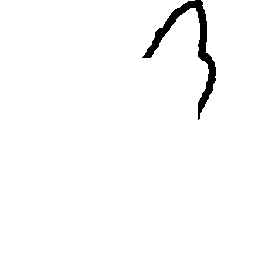
\includegraphics[width=.30\linewidth]{images/ablation_shoes/partial_outline.png}} &
%     \frame{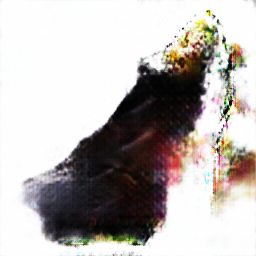
\includegraphics[width=.30\linewidth]{images/ablation_shoes/trained_partial_edges.png}} &
%     \frame{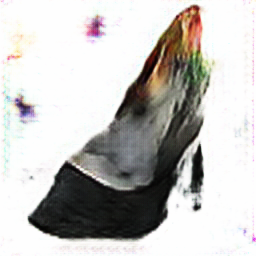
\includegraphics[width=.30\linewidth]{images/ablation_shoes/trained_partial_outlines.png}}
%     \\
%     Input & PE trained & PO trained \\
%     % %
%     % \begin{subfigure}[t]{.30\linewidth}\caption{Input}
%     % \label{fig:basketball_partial}\end{subfigure} &
%     % \begin{subfigure}[t]{.30\linewidth}\caption{PE trained} \label{fig:basketball_full}\end{subfigure} &
%     % \begin{subfigure}[t]{.30\linewidth}\caption{PO trained} \label{fig:soccer_partial}\end{subfigure} \\
%     % %
%     \frame{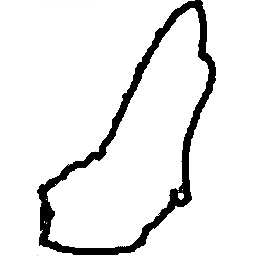
\includegraphics[width=.30\linewidth]{images/ablation_shoes/autocompleted.png}} &
%     \frame{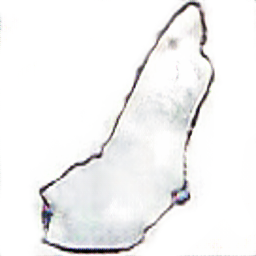
\includegraphics[width=.30\linewidth]{images/ablation_shoes/pretrained_test_autocompleted.png}} &
%     \frame{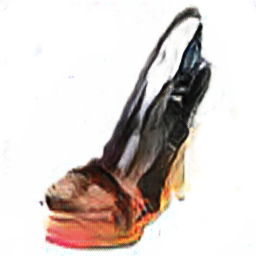
\includegraphics[width=.30\linewidth]{images/ablation_shoes/test_autocompleted.png}} 
%     \\
%     Input & FE trained & FO trained \\
%     % \begin{subfigure}[t]{.30\linewidth}\caption{\textbf{Completion}} \label{fig:soccer_full}\end{subfigure} &
%     % \begin{subfigure}[t]{.30\linewidth}\caption{FE trained}\label{fig:cupcake_partial}\end{subfigure} &
%     % \begin{subfigure}[t]{.30\linewidth}\caption{\textbf{FO trained}} \label{fig:cupcake_full}\end{subfigure}\\
% \end{tabular} \\
% \normalsize
% \vspace{-2mm}
%     \caption{\textbf{Efficacy of outlines:} Networks trained on partial edges (PE) produce worse quality results than those trained on partial outlines (PO) when applied to real human input (top). Similarly, an appearance synthesis model trained on full edges (FE) does not work as well as a network trained on full outlines (FO) when given simplified sketches as input (bottom).}
%     \label{fig:ablation_partialedge_full_outline}
% \end{figure}


\subsection{Insights on Gating Mechanism}
We demonstrate the intuition behind this type of gating by a toy experiment in ~\figref{fig:onedexperiment}, where a generative network models a 1D mixture of Gaussians, comprised of five components. 
For this test, the generator and discriminator architectures consist of only residual blocks, where each residual block is composed of fully connected layers. 
Additional details are in the supplementary material. 
%
The generator is conditioned on a latent vector $z$ and is trained to approximate the distribution, as seen in Fig.~\ref{fig:onedexperiment} (left). 
Removing a single residual block, in the spirit of~\cite{veit2016residual}, leads to the disappearance of a mode from the predicted distribution. 
Removal of another block leads to further removal of another mode, as seen in Fig.~\ref{fig:onedexperiment}  (mid, right). 
This motivates the gating network, which enables the network to learn which blocks (or more specifically, which channels) to attend to for each object class. %It increases the participation of the condition $({\bf y})$ in the generation process which in turn helps the network to effectively disentangle different object classes.
%This experiment shows an encouraging result, suggesting that residual blocks decompose naturally into modeling parts of a distribution.





% \section{Method}
% Interactive Image Generation can be thought of as a sequence of constraints given by the user and the subsequent addition of more constraints based on the geometry or texture constraints provided by the user. In such a constraint based setting a Generative Model has the freedom to choose how to generate a realistic real image honoring the constraints and allowing the freedom to generate as realistically as possible in the unconstrained areas. A system which can generate realistic final images starting from few strokes acting as constraints and honoring constraints at all times would be interactive provided we have fast enough feedforward processing through the network.

% \paragraph{Preliminaries:}
% We can formalize the process of user interaction at the different instances of the interaction, each stroke image at the $i^{th}$ step of the user interaction is $S_i$ representing the user constraints expressed at the $i^{th}$ step of the generation process. $S_i$ can be expressed as a subset of strokes from the set of edges $E$ or from the set of outlines $O$ . $C_i$ is the automatically completed constraint image, completed from the Stroke Image $S_i$ . $G_i$ is the generated image generated by the network after the $i^{th}$ constraint addition step.

% \paragraph{Naive Approaches:}
% As introduced in pix2pix \cite{isola2016image2image} $S_i$ could be from the set of edge maps $E$ but as shown in the experiments section the automatic completion of the constraint image $C_i$ and the subsequent generated image $G_i$ becomes hard in this setting. For instance in case of a partial sketch it'd be hard to discern whether a partial edge is part of the outline of the object or just a texture stroke inside the image hence hindering in the task of interactive image generation. Another naive approach could be to represent the constraint image $S_i$ as a partial outline and generate the full image from the partial outline. There's a reduction in the quality of generations achieved apart from the fact that the automatically completed constraint image $C_i$ further guides the user for better edits to the final image thus granting more control on the generation process.

% \paragraph{Approach:}
% We adopt a two step approach, and restricting the constraint sketches $S_i$ to be from the set of outlines $O$. The first step constitutes of the automatic completion of the constraint sketch $C_i$ from $S_i$ which has to honor the constraints the user has already made in $S_i$ and make sure that the completed constraint sketch $C_i$ is a valid constraint sketch from the domain of valid constraint outlines $O$. We start experiments on the existing datasets of handbags \cite{zhu2016generative} and shoes \cite{yu2014fine}. In these settings the outline would be enough to discern whether the user would like to generate a handbag or a shoe but moving forward in the direction of interactive image generation the user would like to have the option of generating multiple classes and not just a single class. Moving onto multiple classes poses the additional challenge that multiple classes might have similar outlines for instance circular objects such as soccerballs, basketballs and moons have similar outlines which are quite circular. In such a scenario the input constraint sketch $S_i$ or the automatically completed outline $C_i$ is not enough to guide the generation towards the correct class $y$ for the generation. Traditional Image to Image settings fail in proper injection of high dimension information in terms of the source image $S_i$ or $C_i$ with low dimensional class-conditioning information $y$. To properly condition the network in this setting with the class $y$ we introduce a gating hypernetwork \cite{karras2018style} which would be described in the next section.

% \section{Gated Generative Adversarial Network}
% \label{sec:methods}
% We consider image-to-image translation problems, mapping input image $A$ to output $B \in \mathds{R}^{h\times w\times 3}$, with the benefit of a conditioning vector ${\bf y} \in \mathds{R}^{d}$. We learn this mapping with multilayer generator $\mathcal{G}(A,{\bf y})$ to produce output $\widehat{B}$. We refer to the feature map at each channel as $X_l\in \mathds{R}^{h_l\times w_l\times c_l}$, where $h_l \times w_l$ is the spatial size of the feature map, and $c_l$ is the number of channels in the layer. 
% % The total channels in the network is $C = \sum_l C_l$. 
% The conditioning vector ${\bf y}$ can be categorical, expressed as a 1-hot vector, or a continuous vector. 
% % , ground truth output $B \in \mathds{R}^{H\times W\times 3}$, generator $\mathcal{G}$, output $\widehat{B}=\mathcal{G}(A,y)$.
% % \subsection{Conditioning injection variants}
% The way that ${\bf y}$ is integrated into the network plays a critical role. We systematically explore several variants, as illustrated in Fig.~\ref{fig:arch-inj}.

% % There are many ways that the conditioning vector $\bf y$ can be integrated into the network. 

% \subsection{Naive concatenation}
% The most straightforward method is to spatially replicate the vector into a tensor of appropriate size and concatenate it to the input layer~\cite{zhu2017toward,choi2017stargan}. A potential weakness
% % of concatenating at the {\em input only}
% is the large distance between the conditioner and the output, which can lead to the generator easily ignoring the conditioner during learning. A previously explored solution~\cite{zhu2017toward} is to simply concatenate the conditioner into every layer.

% \subsection{Recovering the conditioning vector}

% % \paragraph{Auxiliary classifier or latent regressor for conditioning vector recovery}
% A technique for encouraging adherence to the conditioner is through the objective function. As seen in Fig.~\ref{fig:arch-inj}, a hypernetwork $\mathcal{Q}$ predicts conditioner from output image $\widehat{B}$. 
% % A loss is added to the optimization between ground truth $y$ and predicted $\hat{y}$, and has been explored in 
% The added loss between ground truth ${\bf y}$ and predicted $\hat{ {\bf y}}$ encourages the output to contain information about the conditioner. This has been previously explored in both the class-conditional~\cite{odena2016conditional,choi2017stargan,salimans2016improved} and latent code-conditional settings~\cite{chen2016infogan,donahue2016adversarial,zhu2017toward}. In our experiments, we find that this technique improves upon naive concatenation. We further explore a complementary approach, modifying the architecture of the main generator.

% % \ow{what is the problem with the above approach that leads us to propose the next}
% % \eli{I added a sentence but maybe we can say something stronger? Did we ever try ACGAN on the multi-class task? If yes and it didn't work, maybe mention here?}

% \subsection{Conditioning with Soft-Gating (Proposed)}
% \paragraph{Conditioning with Soft-Gating (Proposed)}
% %The methods above do not fundamentally modify the structure of the network. 
% In ResNets, an input feature tensor $X_l$ is modified by function $X_{l+1} = X_l+\mathcal{H}_l(X_l)$.
% Changes in resolution are obtained by upsampling before or downsampling after the residual block.
% We investigate multiple variants of the \textit{learned} gating network, as illustrated in Fig.~\ref{fig:arch-gate}.
% For visual clarity, we omit the layer subscript $l$ in feature tensor $X_l$, residual subnetwork $\mathcal{H}_l$, and the gating parameters $\alpha_l, \beta_l$.

% We begin by predicting a scalar $\alpha$ using a learned network $\mathcal{F}({\bf y})$ for each layer of the network:

% % We now begin to describe our model which we call Gated Generative Adversarial Networks (GAN-Gate). It is primarily based on an interesting experiment whereby \cite{veit2016residual} showed that the residual networks behave as an ensemble of several shallower networks, and removing a few residual blocks at test time performed highly competitive to the original network itself. This implies that, perhaps, given a GAN architecture with residual blocks as its components, it is possible to {\em automatically} learn a mixture of shallower networks {\em conditioned} on the modes of the data distribution or the tasks we are interested in. This is exactly the objective that GAN-Gate achieves. More precisely, it automatically learns a mixture of shallower networks where each mixture component (a shallow network) is focused on generating data either from a mode or a task; depending on whether we are interested in {\em intraclass} or {\em interclass} variations. To this end, we first propose an architecture for GANs entirely based on residual blocks which is capable of generating highly competitive samples form image-to-image translation task compared to other baselines. Then, we propose to use a simple yet powerful {\em gating mechanism} over a subset of residual blocks where the gating automatically decides which blocks to {\em focus on} for a given condition. Note, this gating is learned automatically from the data. In the end, we also show that the gating mechanism provides an effective way to maximize mutual information in the {\em InfoGAN} objective, which otherwise was not possible.

% \vspace{-2mm}
% \begin{equation}
% X + \alpha \; \mathcal{H}(X), \text{where } \alpha \in [0,1]
% \end{equation}

% If the conditioning vector ${\bf y}$ has no use for a particular block, it can predict $\alpha$ close to zero, and effectively switch off the layer.
% % , and use that layer instead for other classes.
% During training, blocks within the main network can transform the image in various ways, and $\mathcal{F}$ can modulate such that the ``right" blocks are selected. We can also apply the operation channel-wise, using a vector {\boldmath$\alpha$}: % This is denoted as follows:

% \vspace{-4mm}
% \begin{align}
% X + \mbox{\boldmath $\alpha$} \odot \mathcal{H}(X), \text{where } \mbox{\boldmath $\alpha$} \in [0,1]^c 
% \end{align}

% Symbol $\odot$ respresents channel-wise multiplication. This provides additional degrees of freedom, allowing specific channels to be switched ``on" or ``off". We make the corresponding changes in the discriminator as well. 
% %Soft-gating has been explored by Veit et al.~\cite{veit2018adaptive} in a classification setting. 
% Intuitively, in GANs, this can enable the discriminator to select blocks which effectively judge whether generations are real or fake, conditioned on the class input.
% % Via accurate gradients backpropagated to the generator it also enables the generator to generate class conditioned high resolution image samples.
% Some blocks can be shared across regions in the conditioning vector, whereas other blocks can specialize for a given class.

% We empirically find that channel-wise gating provides the strongest results. 
% For completeness, we additionally explore incorporating shifting after the soft-gating, either block-wise using a scalar $\beta \in [-1,1]$ per layer, or channel-wise using a vector $\mbox{\boldmath $\beta$} \in [-1, 1]^c$ per layer.

%\rz{sentence summarizing why or how}
% \begin{equation}
% \text{AdaIn}(x, \alpha, \beta) = \alpha \big(\frac{x-\mu(x)}{\sigma(x)}\big)+\beta
% \label{eqn:adain}
% \end{equation}

% AdaIn layers perform a similar gating task. An Instance Normalization~\cite{ulyanovinstance} (IN) is applied before scaling and shifting the feature distribution. We constrain each element of {\boldmath $\alpha$} and {\boldmath $\beta$} in $[-1, 1]$\footnote{constraining between \( [0, 1] \) did not provide the best empirical results.}.

% \vspace{-2mm}
% \begin{equation}
% X + \mbox{\boldmath $\alpha$} \odot \text{IN} (\mathcal{H}(X)) + \mbox{\boldmath $\beta$}
% \end{equation}

% % \begin{figure*}[t]
% %     \centering
% %     \addSubFigThird{Picture2}{Ground Truth Distribution }{fig:1d_ground} 
% %     \addSubFigThird{Picture33.png}{Generated Samples from the trained Generator}{fig:1d_gen} 
% %     \addSubFigThird{Picture3.png}{Generated Samples from the trained Generator with one of the blocks removed}{fig:1d_gen_rem} 
% %     \caption{{\bf 1D Mixture of Gaussians experiment}}
% %     \label{fig:onedexperiment}
% %     \vspace{-3mm}
% % \end{figure*}


% \begin{figure*}[t]
%   \centering
%   \begin{minipage}[t]{0.48\linewidth}  
%   \centering
%   \resizebox{0.9\linewidth}{!} {
%   \setlength{\tabcolsep}{6pt}
%   \begin{tabular}{l c c c c}
%   \toprule
%     \multirow{3}{*}{\textbf{Method}} & \multicolumn{2}{c}{ {\bf SkinnyResNet}} & \multicolumn{2}{c}{ {\bf EncDec}} \\ \cmidrule(l){2-3} \cmidrule(l){4-5}
% % 	& \textbf{Accuracy} & \textbf{Realism} & \textbf{Accuracy} & \textbf{Realism} \\
% 	& Class. & AMT Fool. & Class. & AMT Fool. \\
% 	& Acc [\%] & Rate [\%] & Acc [\%] & Rate [\%] \\ \midrule
% % 	\cmidrule(l){1-1} \cmidrule(l){2-3} \cmidrule(l){4-5}
%     Ground truth & 100.0 & 50.0 & 100.0 & 50.0 \\ \midrule
%     1 gen/class & \textbf{\textit{97.0}} & 17.7$\pm$1.46 & -- & -- \\ \midrule
%     Concat (In)	& 62.6 & 15.0$\pm$1.4 & 39.2 & 7.5$\pm$1.06 \\ 
%     Concat (All) & 64.5 & 15.3$\pm$1.41 & 51.4 & 5.4$\pm$0.88 \\ \midrule
%     Cat(In)+Aux-Class & 65.6 & 14.5$\pm$1.5 & -- & -- \\ 
%     Cat(All)+Aux-Class & 67.0 & 19.7$\pm$1.42 & -- & --\\ \midrule
%     BlockGate(+bias) & 89.6 & 19.6$\pm$1.34 & -- & --\\ 
%     BlockGate & {\bf 99.6} & 17.3$\pm$1.61 & -- & --\\ 
%     AdaIn & 94.5 & 14.9$\pm$1.47 & -- & --\\ 
%     ChanGate(+bias) & 94.1 & 14.8$\pm$1.43 & -- & --\\ 
%     ChanGate & \textbf{\textit{97.0}} & {\bf 23.4$\pm$1.99} & 92.7 & 14.1$\pm$1.48 \\ 
% 	\hline
% 	\end{tabular} } 
%   \end{minipage}\begin{minipage}[]{0.48\linewidth}
%   \centering
%   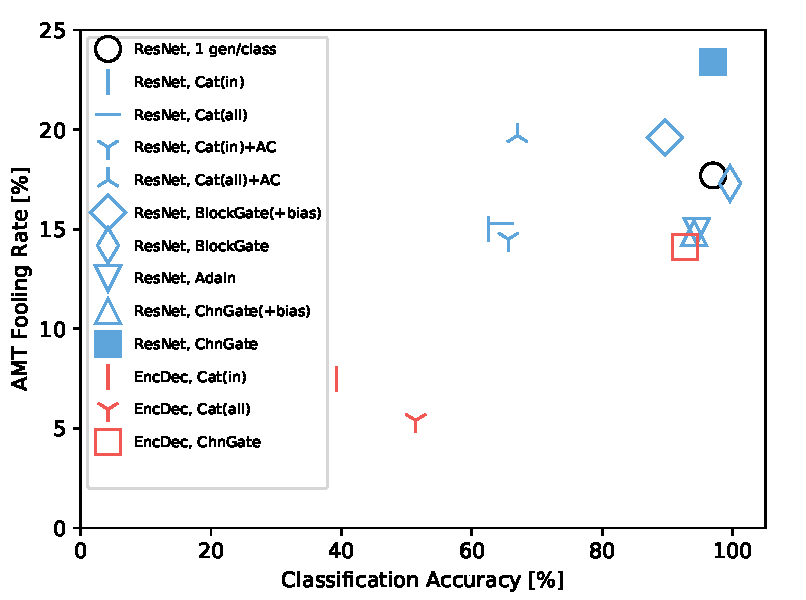
\includegraphics[width=.9\linewidth]{paper_images/gen_real_vs_acc.pdf} 
%   \end{minipage}
%   \caption{\small {\bf Accuracy vs Realism on Outline$\rightarrow$Image task.} We measure generation accuracy by using a pretrained network to check whether the generated image is of the correct class and realism using the user-judged real vs. fake test from ~\cite{zhang2016colorful,isola2016image2image} conducted on Amazon Mechanical Turk (AMT). Higher is better for both metrics. Our SkinnyResNet architecture outperforms the Encoder-Decoder network, inspired by MUNIT~\cite{huang2018multimodal}. We perform a thorough ablation on our architecture, and find that channel-wise gating achieves high accuracy and higher realism. The right figure shows the correlation between the two tasks.
%   \vspace{-4mm}
%   }
%   \vspace{-3mm}
%   \label{fig:acc_vs_real}
% \end{figure*}


% % \subsection{Information Theoretic Benefits of Gating}
% \subsection{Effective Conditioning Injection as Mutual Information Preservation}
% \label{sec:infoGAN} 
% Injecting ${\bf y}$ at various layers essentially glues the generation with the conditioning.
% This helps in avoiding the pathological situation whereby disentanglement over the classes or modes suffer due to an easier approximation, $G(A,y) \approx G(A), \forall y$, learned by the generator. This can be better understood using the {\em data processing inequality}~\cite{cover2012informationTheory}. For any sequential transformation process (\eg feedforward neural networks) over a random variable $y \to f_1(y) \to  x$ (could be of any length); the dependence between $x$ and the transformed random variable decreases as the separation increases. 
% This implies that the mutual information $I(x, f_1(y)) \geq I (x, y)$. Since injection at multiple layers brings ${\bf y}$ closer to the generation $G(A,y)$, it is straightforward to conclude that $I_{Gate}(G(A,y), y) \geq I(G(A,y), y)$. Note, training of generator itself tries to make ${\bf y}$ dependent on the generation. Thus, both naive concatenation in all layers and various forms of gating (refer Fig.~\ref{fig:arch-inj} and ~\ref{fig:arch-gate}) explicitly help the model to achieve this. However, experimentally we observe better dependence when the injection is learned using our gating mechanism. %We also show in the experiment (Sec.~\ref{sec:multimodal}) that with gating, InfoGAN produces diverse generations for image-to-image translation, which otherwise was not possible as the naive conditioning (input concatenation) eventually gets absorbed in the generation making it agnostic to variations in the condition.
% A similar approach has recently been suggested to avoid latent collapse in VAEs~\cite{Dieng18skipVAE}. 

% \pd{not sure how to justify that gating is better using this argument. however, this argument does justify that injection matters. also, the mutual information argument is stronger in case of infoGAN. open to suggestion.}

% \subsection{Improvement on InfoGAN}
%\subsection{Improving the Effectiveness of InfoGAN}
%\label{sec:infoGAN} \rz{need to tie into previous section - this is a special setting of latent regressor}
%InfoGAN\cite{chen2016infogan} has shown impressive results in unconditional image generation where the objective is to maximize the mutual information between the generations $G(z,c;\theta_g)$ and the latent codes $c$, along with generating `real' looking samples. Intuitively, mutual information is maximized if different latent codes allow diverse generations, making the generation and the latent code dependent. However, in the conditional generation situation, where the condition $y$ is highly informative, for example an image, it has been empirically shown that irrespective of how much the noise $z$ or the latent code $c$ is being modified, InfoGAN still suffers from the {\em mode-colslapse} issue\cite{ghosh2017multi}. Thus, fails to generate diverse generations for an extremely important and challenging task of image-to-image translation. For brevity, below we provide the objective function of the generator for the conditional variant of InfoGAN ($z$ removed to avoid clutter):
%\begin{align}
%\label{eq:infoGAN-gen}
%\min_{\theta_g} \log (1 - D(G(y,c; \theta_g); \theta_d) - \lambda \; I (G(y,c; \theta_g), c)
%\end{align}
%%Note, since we only modify the generation process, the objectives of the Q-network and the discriminator is not being discussed here. 
%Generally mode-collapse is the result of the following approximation $G(y,c; \theta_g) \approx G(y; \theta_g), \forall c$. Even though the mutual information term should make $G(y,c;\theta_g)$ and $c$ dependent, it turns out that this is not the case in practice. We advocate the objective function of InfoGAN, however, we hypothesize that the lack of participation of $c$ in the generation process does not allow it to make the generated samples and the latent codes dependent on each other. The gatings, however, resolves this issue by making $c$ an active part of the generation process. Also, from the well known {\em data processing inequality}, \eli{need a citation here!} for any sequential transformation process (\eg feedforward neural networks) over a random variable $c \to f_1(c) \to f_2(f_1(c)) \to x$ (could be of any length); the dependence between $x$ and the transformed random variable decreases as the separation from $x$ increases. This implies $I(x, f_2(f_1(c)) \geq I (x, f_1(c) \geq I (x, c)$. Since the gating function brings $c$ closer to $G(y,c;\theta_g)$, it is straightforward to see that the above inequality implies $I_{Gate}(G(y,c;\theta_g), c) \geq I(G(y,c;\theta_g), c)$. Thus, gating allows the objective to maximize mutual information in a much more effective way than without it. We validate this experimentally by showing that just with gating, InfoGAN is able to produce diverse plausible samples for the image-to-image translation task, which otherwise was not possible.

% \subsection{Interclass Variability using GAN-GATE}
% \label{sec:interclass}
% %As discussed in Section~\ref{sec:infoGAN}, the InfoGAN objective along with the gating for the generator effectively captures the intraclass variability. 
% Since intraclass variability is something that requires automatic disentanglement, as the ground-truth for this is not provided (modes unknown), an InfoGAN type objective is a suitable choice for this (see Section~\ref{sec:infoGAN}). However, for the interclass variability, the ground-truth already provides the task or the class id (\eg, `cat', `dog' \etc) during training. Therefore, there is no need for the network to automatically disentangle them. This avoids the requirement of the mutual information component. To this end, we use gating in both generator and the discriminator to capture interclass variability. 

% The gating in the generator, similar to the arguments provided in Section~\ref{sec:infoGAN}, makes the generation process highly dependent on the class condition. However, providing class-conditional gating for the discriminator enforces it to learn a particular subnetwork for a task to decide whether it is real or fake. This, in turn, via accurate gradient back-propagation provides informative gradients to the generator that enables it to generate class conditioned high resolution image samples. Intuitively, the discriminator distributes some common functions between the different classes to some of these shared residual blocks which are activated for all classes while the rest of the transformations it distributes in a non-overlapping manner to some specific residual blocks of the discriminator network. Such a concept can not only be used for the discriminator but in many settings where the conditioning variable is known, for example some plausible applications can be the Q network in InfoGAN\cite{chen2016infogan} or the Conditional Inference Network in a CVAE \cite{sohn2015learning}. \figref{fig:gru_dis} illustrates the concept in the setting of the conditional discriminator. Some other extensions such as affine gating per residual block and channel wise gating with its affine counterpart exists as well apart from Adaptive Instance Normalization(AdaIN) \cite{huang2017arbitrary}.


% ***** RZ *****


% rz - I cut this from preliminary section

% One aspect of residual networks is that information can bypass layers, forming essentially an ``ensemble'' of several shallower networks.
% Veit et al.~\cite{veit2016residual} showed in a classification setting, that classification performance is largely maintained even when fully removing some residual blocks.
% We investigate whether this aspect can lead to more efficient parameter usage for multi-class image generation, by using fully residual networks for both generator and discriminators in a GAN network.
% Instead of fully removing residual blocks, we evaluate a number of soft-gating mechanisms.

%with a whereby a hypernetwork gets the condition modulates the feature activations of the residual blocks i.e. the output of the standard residual block was modified from $x+f(x)$ to  $x+\alpha . f(x)$ where the set of alphas for each of the residual block is predicted by the hypernetwork. 

% \paragraph{Relationship to conditioning}
% This approach can be seen as form of conditioning. 
% Conditioning by concatenation is a weak form of conditioning because by information theoretic principles, the deeper the network the lesser mutual information is preserved between the conditioning input and the output of the network. To mitigate this issue some other solutions such as the projection discriminator \cite{miyato2018cgans} have been proposed and our residual gate selection block on the discriminator is along similar lines. 






% \paragraph{Architecture}

% \section{Gated Residual Block based Generator}
% Inspired by the incision experiments performed on the generator whereby removal of certain blocks led to the removal of particular modes from the data distribution, our model consists of a main network which is oblivious to the condition provided to the network, while another hypernetwork only receives the condition and has to predict which block should be used to what extent. More precisely, the $i^{th}$ residual block now receives an extra input $\alpha_i$ alongside the usual $x$ and the output of the gated residual block is $x+\alpha_i*f_i(x)$ rather than the standard $x+f_i(x)$. The $alpha_i$s are predicted via another hypernetwork which only receives the condition and has no idea about the input being received by the main block. The interpretation of the above is that if some block doesn't have to be used for a particular class then the hypernetwork can just choose the $alpha_i$ close to 0 and effectively that block is switched off. The intuition is that the hypernetwork has to first understand the transformations that the different residual blocks in the generator are learning, then start modulating it such that conditioned on the class the required blocks are chosen to the right extent such that the resulting sequence of transformations corresponds to realistic images from that particular class. Its related to FILM \cite{perez2017film} albeit it does feature wise transform and has to predict more parameters than a single number per block. \figref{fig:gru_gen} illustrates the concept in the setting of the conditional generator. Some other extensions such as affine gating per residual block and channel wise gating with its affine counterpart exists as well apart from the well known Adaptive Instance Normalization \cite{huang2017arbitrary} . The varied forms of gating could be applied to the Infogan setup with the gate prediction block receives the randomly sampled latent as input to decide the gates on the various blocks while the Q network trying to reconstruct back the latent that was passed.
 
% \section{Gated Residual Block based Discriminator}

% Based on a similar principle as the Generator, the Discriminator can also be equipped with gated residual blocks whereby each residual block would compute $x+\alpha_i*f_i(x)$ in place of the standard $x+f_i(x)$ where each $alpha_i$ is predicted by another hypernetwork which gets the condition that which class is the network currently judging for real/fake. Its intriguing that with just the class information the hypernetwork is able to select blocks which effectively guide the discriminator to judge whether its real/fake conditioned on the class. Via accurate gradients backpropagated to the generator it also enables the generator to generate class conditioned high resolution image samples. Intuitively, the discriminator distributes some common functions between the different classes to some of these shared residual blocks which are activated for all classes while the rest of the transformations it distributes in a non-overlapping manner to some specific residual blocks of the discriminator network. Such a concept can not only be used for the discriminator but in many settings where the conditioning variable is known, for example some plausible applications can be the Q network in InfoGAN\cite{chen2016infogan} or the Conditional Inference Network in a CVAE \cite{sohn2015learning}. \figref{fig:gru_dis} illustrates the concept in the setting of the conditional discriminator. Some other extensions such as affine gating per residual block and channel wise gating with its affine counterpart exists as well apart from Adaptive Instance Normalization(AdaIN) \cite{huang2017arbitrary}

% \section{GAN-Gate}
% We now begin to describe our model which we call Gated Generative Adversarial Networks (GAN-Gate). It is primarily based on an interesting experiment whereby \cite{veit2016residual} showed that the residual networks behave as an ensemble of several shallower networks, and removing a few residual blocks at test time performed highly competitive to the original network itself. This implies that, perhaps, given a GAN architecture with residual blocks as its components, it is possible to {\em automatically} learn a mixture of shallower networks {\em conditioned} on the modes of the data distribution or the tasks we are interested in. This is exactly the objective that GAN-GATE achieves. More precisely, it automatically learns a mixture of shallower networks where each mixture component (a shallow network) is focused on generating data either from a mode or a task; depending on whether we are interested in {\em intraclass} or {\em interclass} variations. To this end, we first propose an architecture for GANs entirely based on residual blocks which is capable of generating highly competitive samples form image-to-image translation task compared to other baselines. Then, we propose to use a simple yet powerful {\em gating mechanism} over a subset of residual blocks where the gating automatically decides which blocks to {\em focus on} for a given condition. Note, this gating is learned automatically from the data. In the end, we also show that the gating mechanism provides an effective way to maximize mutual information in the {\em InfoGAN} objective, which otherwise was not possible.

% \subsection{Residual Blocks based GAN Architecture}
% \label{sec:resnet-architecture}
% \pd{Brief overview of our architecture?}
% \subsection{Gated Residual Blocks and its Variants}
% \label{sec:gated-resnet}
% \pd{talk about gating and its variants. relation with FilM etc? Point to Richard's figure and provide some intuitions}
% \subsection{Improving the Effectiveness of InfoGAN}
% \label{sec:infoGAN}
% InfoGAN\cite{chen2016infogan} has shown impressive results in unconditional image generation where the objective is to maximize the mutual information between the generations $G(z,c;\theta_g)$ and the latent codes $c$, along with generating `real' looking samples. Intuitively, mutual information is maximized if different latent codes allow diverse generations, making the generation and the latent code dependent. However, in the conditional generation situation, where the condition $y$ is highly informative, for example an image, it has been empirically shown that irrespective of how much the noise $z$ or the latent code $c$ is being modified, InfoGAN still suffers from the {\em mode-collapse} issue\cite{ghosh2017multi}. Thus, fails to generate diverse generations for an extremely important and challenging task of image-to-image translation. For brevity, below we provide the objective function of the generator for the conditional variant of InfoGAN ($z$ removed to avoid clutter):
% \begin{align}
% \label{eq:infoGAN-gen}
% \min_{\theta_g} \log (1 - D(G(y,c; \theta_g); \theta_d) - \lambda \; I (G(y,c; \theta_g), c)
% \end{align}
% %Note, since we only modify the generation process, the objectives of the Q-network and the discriminator is not being discussed here. 
% Generally mode-collapse is the result of the following approximation $G(y,c; \theta_g) \approx G(y; \theta_g), \forall c$. Even though the mutual information term should make $G(y,c;\theta_g)$ and $c$ dependent, it turns out that this is not the case in practice. We advocate the objective function of InfoGAN, however, we hypothesize that the lack of participation of $c$ in the generation process does not allow it to make the generated samples and the latent codes dependent on each other. The gatings, however, resolves this issue by making $c$ an active part of the generation process. Also, from the well known {\em data processing inequality}, for any sequential transformation process (\eg feedforward neural networks) over a random variable $c \to f_1(c) \to f_2(f_1(c)) \to x$ (could be of any length); the dependence between $x$ and the transformed random variable decreases as the separation from $x$ increases. This implies $I(x, f_2(f_1(c)) \geq I (x, f_1(c) \geq I (x, c)$. Since the gating function brings $c$ closer to $G(y,c;\theta_g)$, it is straightforward to see that the above inequality implies $I_{Gate}(G(y,c;\theta_g), c) \geq I(G(y,c;\theta_g), c)$. Thus, gating allows the objective to maximize mutual information in a much more effective way than without it. We validate this experimentally by showing that just with gating, InfoGAN is able to produce diverse plausible samples for the image-to-image translation task, which otherwise was not possible.



